\documentclass[english,11pt]{article}
\usepackage[paperwidth=210mm,paperheight=297mm,margin=15mm]{geometry}
%\usepackage{algorithmic,algorithm}
\usepackage{psfrag,subfigure}
\usepackage{epsfig,multirow,color,url,colortbl,xcolor}
\usepackage[latin1]{inputenc}
\usepackage{amssymb,fancyhdr,epsfig,psfrag,tabularx,amsmath,theorem,pifont}
%\usepackage[brazil]{babel}
%\usepackage{matlab-prettifier}
\usepackage[bw,framed]{mcode}


\newcommand*{\colorboxed}{}
\def\colorboxed#1#{%
  \colorboxedAux{#1}%
}
\newcommand*{\colorboxedAux}[3]{%
  % #1: optional argument for color model
  % #2: color specification
  % #3: formula
  \begingroup
    \colorlet{cb@saved}{.}%
    \color#1{#2}%
    \boxed{%
      \color{cb@saved}%
      #3%
    }%
  \endgroup
}

% configuration of tables with gray background
\definecolor{gray1}{gray}{0.95}
\newcolumntype{A}{>{\columncolor{gray1}}c}
\definecolor{defbkgd}{gray}{0.95}
\doublerulesepcolor{defbkgd}


\newcommand\hi{\hspace*{\parindent}}
\newcommand\vi{\vspace{.5cm}}


\theoremstyle{break} \theorembodyfont{\small\rm}
\newtheorem{exemplo}{\bf Example}

\theorembodyfont{\rm}
\newtheorem{propri}{\bf Property}

\theorembodyfont{\rm}
\newtheorem{teorema}{\bf Theorem}

\theorembodyfont{\rm}
\newtheorem{definicao}{\bf Definition}

\theorembodyfont{\rm}
\newtheorem{rem}{\bf Remark}

\theorembodyfont{\rm}
\newtheorem{lema}{\bf Lemma}

\theorembodyfont{\rm}
\newtheorem{algorithm}{\bf Algorithm}

\newcounter{Iexctr}
\newenvironment{Iexemplo}[1]
{\stepcounter{Iexctr} \begin{center} \begin{quote} \small {\bf
Exemplo~\arabic{Iexctr}: {#1}} \\} {\hspace*{\fill}\nolinebreak[1]
\end{quote} \end{center}}

\newenvironment{Pexemplo}
{\begin{center} \begin{quote} \small \begin{exemplo}}
{\hspace*{\fill}\nolinebreak[1]
\end{exemplo}
\end{quote} \end{center}}

\newenvironment{Ppropri}
{\begin{propri}} {\hspace*{\fill}\nolinebreak[1]
\end{propri}
}

\newenvironment{Pteorema}
{\begin{teorema}} {\hspace*{\fill}\nolinebreak[1]
\end{teorema}
}

\newenvironment{Pdefi}
{\begin{definicao}} {\hspace*{\fill}\nolinebreak[1]
\end{definicao}
}

\newenvironment{remark}
{\begin{rem}} {\hspace*{\fill}\nolinebreak[1]
\end{rem}
}

\newenvironment{Plema}
{\begin{lema}} {\hspace*{\fill}\nolinebreak[1]
\end{lema}
}

\newenvironment{Palgorithm}
{\begin{algorithm}} {\hspace*{\fill}\nolinebreak[1]
\end{algorithm}
}

\newenvironment{proof}{\noindent{\bf Proof:}}{\null\hfill $\rule{1.5mm}{1.5mm}$}

\newcommand{\Hd}{{\mathcal{H}}_{2}}
\newcommand{\Hi}{{\mathcal{H}}_{\infty}}

\begin{document}

%\selectlanguage{english}

\title{Manual of ``The Robust LMI Parser'' -- Version 3.0}
%\thanks[footnoteinfo]{Supported by CNPq, FAPESP and CAPES-COFECUB.}
        
\author{Cristiano M. Agulhari\thanks{Federal University of Technology of Paran\'{a} -- UTFPR, Campus Corn\'{e}lio Proc\'{o}pio, PR. E-mail: agulhari@utfpr.edu.br}, 
Alexandre Felipe\thanks{School of Electrical and Computer Engineering, University of Campinas -- UNICAMP,  13083-852, Campinas, SP, Brazil. E-mails: 
o.alexandre.felipe@gmail.com, \{ricfow,peres\}@dt.fee.unicamp.br}, Ricardo C. L. F. Oliveira\footnotemark[2], and Pedro L. D. Peres\footnotemark[2] }

%TODO: Explicar a funcao ``coefs'' !!!!!!


\maketitle
%\selectlanguage{english}

\begin{abstract}                          % Abstract of not more than 250 words.
The ROLMIP (Robust LMI Parser), built to work under MATLAB jointly with YALMIP, is a toolbox aimed to ease the 
programming of Linear Matrix Inequality (LMI) relaxations for parameter-dependent LMIs with parameters lying in unit simplexes (or inside known intervals).
Through simple commands, the user is able to define matrix polynomials, as well as to described the desired parameter-dependent LMI conditions in a easy way, considerably reducing
the programming time.
The main commands and definitions are thoroughly explained in this manual.

\end{abstract}

%\end{frontmatter}


\section{Introduction}

In the last decades, problems formulated in terms of Linear Matrix Inequality (LMI)
conditions and solved by Semidefinite Programming (SPD) techniques became more and more
common in several fields related to engineering and applied mathematics. 
Specifically in control theory, the growing
usage of such relevant tools has led to important results on the analysis of systems stability, 
synthesis of robust controllers and filters
for uncertain systems and synthesis of optimal control models, just to name a few problems
\cite{BEFB:94}. 

Accompanying the growth of the usage of LMI optimization, a large number of solvers based on interior point methods
were developed, as well as interfaces for parsing the LMIs, most of them free and easily accessible.
Thanks to such remarkable advance in the computational tools
to define, manipulate and solve LMIs, in many cases one can say that if a problem
can be cast as a set of LMIs, then it can be considered as solved \cite{BEFB:94}. 
Unfortunately, this is not completely true for large scale systems, since LMI
solvers are limited to a few thousands of variables and LMI rows, but progresses
are being made.

Usually, the approach to solve LMIs is decomposed in two steps: first, an interface for parsing the conditions is
used, for example the YALMIP \cite{Lof:04} or the LMI Control Toolbox from
MATLAB \cite{GNLC:95}; then, an LMI solver is invoked to find a solution (if any),
for example SeDuMi \cite{Stu:99}, SDPT3 \cite{TTT:99} or MOSEK~\cite{AA:00}. Some auxiliary toolboxes
may also be used in addition to the parser and solver, for example the SOSTOOLS
\cite{PPSP:04}, which is used to transform a sum of squares problem into an SDP
formulation, GloptiPoly \cite{HL:03c}, used to handle optimization problems
over polynomials, and the R-RoMuLOC~\cite{rromuloc,rromulocconf,romulocconf,ractconf}, a toolbox for the manipulation and
resolution of conditions related to robust multi-objective control.

To motivate the use of ROLMIP consider, for instance, the problem of analyzing the
stability of a discrete-time linear system given by
\begin{equation}\label{eq_discr_system}
 x(k+1) = Ax(k),
\end{equation}
with $x(k) \in \mathbb{R}^n$ being the state vector of the system and $A \in \mathbb{R}^{n \times n}$
being the dynamic matrix. Following the Lyapunov stability theory, such system is stable if and only if
there exists a symmetric matrix $P \in \mathbb{R}^{n \times n}$
such that the LMI
\begin{equation}\label{eq_estab_discr}
 \begin{bmatrix} P & A'P \\ PA & P \end{bmatrix} > 0
\end{equation}
holds. Such LMI can be easily programmed and solved using, respectively, 
any LMI parser and solver available.

Consider now that system (\ref{eq_discr_system}) is affected by uncertainties, i.e., the
system matrix is parameter-dependent and is given by $A(\alpha)$. The robust stability analysis
of such system can be performed by rewriting the LMI condition (\ref{eq_estab_discr}) as
\begin{equation}\label{eq_estab_discr_param}
 \begin{bmatrix} P(\alpha) & A(\alpha)'P(\alpha) \\ P(\alpha)A(\alpha) & P(\alpha) \end{bmatrix} > 0
\end{equation}
but, in this case, (\ref{eq_estab_discr_param}) must hold for all admissible $\alpha$.
In order to transform the parameter-dependent LMI into a finite set of standard
LMIs, some information about $A(\alpha)$ must be added, as well as some structure must
be imposed to the unknown variable $P(\alpha)$.
For instance, consider that $A(\alpha)$ and $P(\alpha)$ have a polytopic structure
\begin{equation}\label{eq_aalfa_politopico}
 A(\alpha) = \sum_{i=1}^N \alpha_i A_i~,~P(\alpha) = \sum_{i=1}^N \alpha_i P_i~,~~ \alpha \in \Delta_N,
\end{equation}
being $A_i$ and $P_i$ the vertices of the respective polytopes, $N$ the number of 
vertices and $\Delta_N$ the set known as unit simplex, given by
\begin{equation}\label{eq_unit_simplex}
 \Delta_N = \big\{ \alpha \in \mathbb{R}^N : \sum_{i=1}^N \alpha_i = 1~,~~ 
\alpha_i \geq 0~,~~ i = 1,\ldots,N \big\}.
\end{equation}
Applying the definition of $A(\alpha)$ and the chosen structure for $P(\alpha)$, given by~\eqref{eq_aalfa_politopico},
to the robust stability condition expressed in the parameter-dependent LMI~\eqref{eq_estab_discr_param}, one gets
the following homogeneous polynomial matrix inequality, of degree $2$ on $\alpha$, 
\begin{multline}\label{eq_poly_lmi}
 \begin{bmatrix} P(\alpha) & A(\alpha)'P(\alpha) \\ P(\alpha)A(\alpha) & P(\alpha) \end{bmatrix} = 
\sum_{i=1}^N \alpha_i^2 \begin{bmatrix} P_i & A_i'P_i \\ P_iA_i & P_i \end{bmatrix} 
+ \sum_{i=1}^{N-1} \sum_{j=i+1}^N \alpha_i\alpha_j \begin{bmatrix} P_i + P_j & A_i'P_j + A_j'P_i \\ P_iA_j + P_jA_i & P_i + P_j \end{bmatrix} > 0. 
\end{multline}

A sufficient
(but not necessary) way to guarantee that (\ref{eq_estab_discr_param}) holds is to impose
that all the matrix coefficients of the monomials are positive definite. This has been done, for instance, in \cite{RP:01b} (discrete-time systems) and \cite{RP:02} (continuous-time systems). 
A less conservative set of conditions
may be obtained by modeling the variable $P(\alpha)$ in (\ref{eq_poly_lmi}) as a
homogeneous polynomial with generic degree $g > 1$ and then imposing the positivity of all
matrix coefficients \cite{OP:06a,BOMP:06b}. Programming these LMIs requires
an \textit{a priori} knowledge on the formation law of the monomials, which depends
on the number $N$ of uncertain parameters and on the degree of the polynomial variable
$P(\alpha)$. In \cite{OP:07a}, a systematic way  to deal with such cases has been developed, but 
in the context of robust LMIs  presenting at most products between two parameter-dependent matrices.
When the LMIs to be solved are more complex and have products involving three or more parameter-dependent 
matrices, a systematic procedure to generate the coefficients of the monomials can be very hard (at least tedious) to be developed.

Consider now that matrix $A(\cdot)$ depends on two parameters, $\alpha$ and $\beta$, being each
parameter contained in an independent unit simplex, \textit{i.e.},
\begin{equation}
 A(\alpha,\beta) = \sum_{i = 1}^{N_1} \sum_{j = 1}^{N_2} \alpha_i \beta_j A_{ij}, ~~~\alpha \in \Delta_{N_1}, \beta \in \Delta_{N_2},
\end{equation}
That is, the parameters $\alpha$ and $\beta$ lie in the multi-simplex $\Omega = \Delta_{N_1} \times \Delta_{N_2}$
(\textit{i.e.}, the Cartesian product of $\Delta_{N_1}$ and 
$\Delta_{N_2}$). Defining
\begin{equation}
P(\alpha,\beta) = \sum_{i = 1}^{N_1} \sum_{j = 1}^{N_2} \alpha_i \beta_j P_{ij},
\end{equation}
then the parameter-dependent LMI to verify the robust stability of the system becomes
\begin{equation}
 \begin{bmatrix} P(\alpha,\beta) & A(\alpha,\beta)'P(\alpha,\beta) \\ P(\alpha,\beta)A(\alpha,\beta) & P(\alpha,\beta) \end{bmatrix} > 0,
\end{equation}
which is a completely different case than the one in~\eqref{eq_poly_lmi}, with $A(\alpha)$ described
in terms of one simplex as in~\eqref{eq_aalfa_politopico}, therefore with a different formation law for the monomials.
This illustrates that each new case requires the manipulation of different polynomials and such
task, as well as programming the resulting LMIs, can be tedious, time-demanding and
also a source of programming errors.

The toolbox described in this manual, called Robust LMI Parser\footnote{Available
at \url{http://rolmip.github.io}}, intends to 
overcome these problems by automatically computing all the coefficients of the monomials of a given 
parameter-dependent LMI. Those coefficients define the set of sufficient LMI conditions to be programmed. 
A feasible solution assures that the parameter-dependent LMI conditions are verified for the entire domain of uncertainty.  
The toolbox is developed for MATLAB and works jointly with YALMIP,
returning the entire set of LMIs through a few simple commands that describe the 
structure of the known matrices and variables involved in the parameter-dependent LMIs to be investigated. 

\section{Installation notes}

ROLMIP was built on the top of YALMIP \cite{Lof:04}, a freely distributed general purpose optimization parser MATLAB toolbox.
Therefore the first step before using ROLMIP is to download\footnote{\url{https://yalmip.github.io/download/}} and install YALMIP.

The ROLMIP installation is simple: just unzip the installation file ({\tt robust\_lmi\_parser.zip}) and then add the decompressed folder on MATLAB's path. 
To check if ROLMIP is working properly, run the script {\tt rolmiptest.m}.

In order to solve the semidefinite problems proposed in this manual, it is necessary to install a proper solver. Among the several solvers publicly available,
we recommend the following:
\begin{itemize}
 \item SeDuMi (\url{http://sedumi.ie.lehigh.edu/})
 
 \item MOSEK (\url{http://www.mosek.com/})
 
 \item SDPT3 (\url{http://github.com/SQLP/SDPT3})
\end{itemize}

The examples and outputs shown in this manual were generated by using YALMIP R20180612 with SeDuMi 1.3, operating under
MATLAB R2015a.

%\mcode{ 'AAA' }

\subsection{Notes on Version 3.0}

The current version is considerably different from the previous ones, mainly due to the introduction of a
new variable type, named \texttt{rolmipvar}. With this modification, the commands and definitions are more
straightforward and easy to use and understand, and even the computational time necessary to parse the parameter-dependent LMIs has been optimized. 
We strongly suggest the use of \texttt{rolmipvar} instead of the old commands \texttt{poly\_struct} and \texttt{parser\_poly}.
However, such old commands are still implemented and even somewhat improved in the current version, and the MATLAB routines that already
use ROLMIP continue to work.

Concerning specifically the automatic creation of executable MATLAB files: the latter version 
provided a set of procedures (using the old commands \texttt{poly\_struct} and \texttt{parser\_poly})
whose objective was to generate automatically MATLAB .m files, saving computational time if a
set of conditions need to be executed several times. Such features are still part of ROLMIP, but not yet
adapted to work using the \texttt{rolmipvar} variables included in the present version. Please
refer to the manual of the previous version for further details.

\subsection{YALMIP compatibility issues}

Since YALMIP does not recognize the classes of ROLMIP in its source code, some compatibility issues may occur. Usually, such
problems may happen if \texttt{sdpvar} and \texttt{rolmipvar} variables are mixed in the same expression. Thus,
in order to avoid conflicts, we strongly suggest that
the script under development be solely based on \texttt{rolmipvar} variables. If using
both structures is unavoidable, it is important to guarantee that \texttt{rolmipvar} variables
appear before the \texttt{sdpvar} ones when writing the expressions, as emphasized in Remark~\ref{rem_issues} in Section~\ref{sec_example}.

\newpage

\section{Preliminaries}\label{sec_preliminaries}

ROLMIP currently considers the following assumptions:
\begin{itemize}
\item The polynomial matrices are dependent on parameters that either are 
defined over a unit (or multi) simplex domain, or have known bounds;

\item The number of vertices of a given simplex is always the same, although different
simplex domains may present different numbers of vertices.
\end{itemize}

Several examples illustrating the usage of the commands are
presented throughout the manual. Single commands are displayed using
a font \mcode{similar to the one used in MATLAB} and start with \mcode{>>}.
Fully functional scripts, presented in some examples, are encapsulated
by a \boxed{\mbox{black box}}, while the MATLAB outputs generated by such scripts are
displayed inside a \colorboxed{red}{\mbox{red box}}.



\section{Structure and definition of a polynomial variable}\label{sec_poly_struct}

The main structure of ROLMIP is the \mcode{rolmipvar} class, which
stores the informations regarding the polynomial structure of the parameter-dependent
matrices. Internally, a \mcode{rolmipvar} variable is a structure composed by the following fields:
\begin{itemize}
 \item \mcode{vertices}: Contains the number of vertices of each simplex;
 
 \item \mcode{data}: This field is a vector of elements (stored using the type \mcode{cell array} from MATLAB) that describes all the monomials
 of the variable. Each position of the vector is composed by the fields \mcode{value}, which contains the value
 of coefficient of the monomial, and \mcode{exponent}, describing the exponent of the monomial;
 
 \item \mcode{label}: Informs the label of the variable, which is used mainly for the \LaTeX ~text 
 generation;
 
 \item \mcode{opcode}: Describes how a variable is constructed, either if it is a user-defined variable
 or if it is the result of a previous mathematical operation;
 
 \item \mcode{bounds}: Used only if the polynomial depends on time-varying parameters with known variation rates.
\end{itemize}

The fields of the \mcode{rolmipvar} structure are not directly accessible by the user, and some of them (namely  \mcode{opcode} and 
\mcode{bounds}) are defined only for internal purposes. 
For instance, consider a polynomial matrix $M(\alpha,\beta)$ defined in a multi-simplex domain as
\begin{multline}\label{eq_ex1_M}
  M(\alpha,\beta) = \alpha_1^2\beta_1 M_1 + \alpha_1\alpha_2\beta_1 M_2 + \alpha_2^2\beta_1 M_3 +
  \alpha_1^2\beta_2 M_4 + \alpha_1\alpha_2\beta_2 M_5 + \alpha_2^2\beta_2 M_6  \\ +
  \alpha_1^2\beta_3 M_7 + \alpha_1\alpha_2\beta_3 M_8 + \alpha_2^2\beta_3 M_9,
 \end{multline}
 with $\alpha \in \Lambda_2$ and $\beta \in \Lambda_3$. The internal structure of the related \mcode{rolmipvar} 
 variable is illustrated on Table~\ref{tab_struct_rolmipvar}.
 

\begin{table*}[!ht]
\caption{Structure of the \mcode{rolmipvar} variable representing the polynomial defined in~\eqref{eq_ex1_M}.\label{tab_struct_rolmipvar}}{
\begin{tabular}{|c|c|c|c|c|c|c|} \hline 
\multicolumn{7}{|c|}{\mcode{label} = 'M'} \\
\hline \multicolumn{7}{|c|}{\mcode{vertices} = [2 ~ ~ 3]} \\
\hline \multicolumn{2}{|c|}{\mcode{data(1)}} & \multicolumn{2}{c|}{\mcode{data(2)}} & \multirow{4}{*}{$\ldots$} & \multicolumn{2}{c|}{\mcode{data(9)}} \\
\cline{1-4} \cline{6-7} \multicolumn{2}{|c|}{\mcode{value} = $M_1$} & \multicolumn{2}{c|}{\mcode{value} = $M_2$} &  & \multicolumn{2}{c|}{\mcode{value} = $M_9$} \\
\cline{1-4} \cline{6-7} \mcode{exponent\{1\}} & \mcode{exponent\{2\}} & \mcode{exponent\{1\}} & \mcode{exponent\{2\}} & & 
\mcode{exponent\{1\}}  & \mcode{exponent\{2\}} \\
  $[2 ~0]$ & $[1 ~0~ 0]$ &  $[1~ 1]$ &  $[1  ~ 0 ~0]$ & & 
  $[0 ~2]$ &  $[0~ 0 ~1]$ \\
\hline
\end{tabular}}
\end{table*}


\subsection{Accessing the monomials of a \mcode{rolmipvar} variable}


There are two ways to access the informations of the polynomials:
 \begin{itemize}
 \item Using the index operator (  ) with the exponents of the desired monomial. For instance, to consult the coefficient related
  to the monomial $\alpha_1^2\beta_2$ of the polynomial $M(\alpha,\beta)$ defined in~\eqref{eq_ex1_M}, enter the command
  \[
    \mbox{\mcode{>> M([2 0],[0 1 0]);}}
  \]
  
  \item By using the command 
  \[
    \mbox{\mcode{>> Mi = coeffs(poly);}}
  \]
  which returns a cell structure containing all the coefficients of the monomials from the \mcode{rolmipvar} variable \mcode{poly}.
  In this case, the output contains only the monomials, and not the respective exponents, which can be obtained through the command
  \[
   \mbox{\mcode{>> expMi = exponents(poly);}}
  \]
  The output variable \mcode{expMi} is structured as
  \[
   \mbox{\mcode{expMi\{index\}}}
  \]
  where \mcode{index} corresponds to the coefficient stored in \mcode{Mi{index}}. The structure of \mcode{expMi{index}} is similar 
  to the \mcode{exponent} component shown in Table~\ref{tab_struct_rolmipvar}.


 \end{itemize}
%

\subsection{Defining polynomial variables composed by known matrices in a multi-simplex domain}

Every polynomial variable, regardless if depending on (multi) simplex or bounded parameters, is defined of type \mcode{rolmipvar}. 
The variable definition may be performed using
several different syntaxes\footnote{The syntaxes are somewhat similar to the
\mcode{poly\_struct} command available on prior versions.} depending on how the polynomial is described
by the user, as detailed below.

If the matrix polynomial has known coefficients (as opposed to \mcode{sdpvar}\footnote{Variables used
in YALMIP toolbox.} variables), the 
polynomial variable is obtained by
\[
\mbox{\mcode{poly = rolmipvar(M,label,vertices,degree)}}
\]

The output \mcode{poly} is a \mcode{rolmipvar} variable that fully describes the polynomial. 
The input \mcode{M} contains data about the coefficients and the monomials of the
polynomial to be defined. 
The input \mcode{label} is a string and consists of a name used to refer the
variable, used mainly to generate the {\LaTeX} code of a polynomial through the command \mcode{texify}, presented later. 
The inputs \mcode{vertices} and \mcode{degree} inform, respectively, the number
of parameters (vertices) and the polynomial degrees of the parameters associated to each simplex of the polynomial. If a parameter-independent
matrix is to be defined, then the parameters \mcode{vertices} and \mcode{degree} may be omitted
or set to zero.

For instance, consider that matrix $A(\alpha)$ has the following structure
\[
A(\alpha) = \alpha_1 A_1 + \alpha_2 A_2, ~~\alpha_1 + \alpha_2 = 1, ~~  \alpha_1 \geq 0, \alpha_2 \geq 0
\]
i.e., $A(\alpha)$ is characterized by a polytope of $N = 2$ vertices and is
modeled as a homogeneous polynomial of degree $g = 1$ with parameters in the unit simplex. There are three ways of inputting
the coefficients $A_1$ and $A_2$ through variable \mcode{M}:
\begin{enumerate}
\item Concatenating the matrices $A_1$ and $A_2$;
\[
\mbox{\mcode{>> M = [A1 A2];}}
\]

\item Using \mcode{M} as a cell array;
\begin{equation}\label{eq_cell_array}
\mbox{\mcode{>> M\{1\} = A1; M\{2\} = A2;}}
\end{equation}

\item Informing, in the cell array \mcode{M}, the exponent of the monomial to which each matrix
is related.
\begin{equation}\label{eq_cell_array_expon}
 \mbox{\mcode{>> M\{1\} = \{[1 0],A1\}; M\{2\} = \{[0 1],A2\};}}
\end{equation}
Using this syntax, the exponent of the monomial $\alpha_1^{n_1}\alpha_2^{n_2} \ldots \alpha_N^{n_N}$
is encoded as $[n_1 ~ n_2 ~ \ldots ~ n_N]$. If more simplexes are used, then each cell has
extra elements; refer to Example~2.
\end{enumerate}
Please note that, if the first two ways are used, then every monomial must be defined, 
and the order of elements is important. On the other hand, if the third way is used,
then there is no specific order, and the undefined monomials are set to zero by
default.

Constant matrices may be defined by setting \mcode{vertices} with
the number of vertices for the problem under investigation and \mcode{degree = 0}. However,
the structure will be more complex and may result on more expensive
computations.


\subsubsection*{Example 1}
Consider the polynomial matrix $A(\alpha)$ with degree $g=1$ that represents a polytopic linear system 
with $N = 3$ vertices given by
\[
A(\alpha) = \alpha_1 A_1 + \alpha_2 A_2 + \alpha_3 A_3, ~ ~  \alpha \in \Delta_3,
\]
being
\[
 A_1 = \begin{bmatrix} 1 & 0 \\ 0 & 1 \end{bmatrix}, \quad
 A_2 = \begin{bmatrix} 2 & 0 \\ 0 & 2 \end{bmatrix}, \quad
 A_3 = \begin{bmatrix} 3 & 0 \\ 0 & 3 \end{bmatrix}.
\]
Such a polynomial can be defined using the following script\footnote{Available in the file \texttt{example\_1.m} within the folder \texttt{manual\_examples}.}

%\vspace{0.5cm}%\hspace{2cm}
\begin{minipage}{8.5cm}
\begin{lstlisting}
 %Example 1
 A1 = eye(2);
 A2 = 2*eye(2);
 A3 = 3*eye(2);
 A = [A1 A2 A3];
 polyA = rolmipvar(A,'A',3,1);
\end{lstlisting}
\end{minipage}

\vi
The contents of the \mcode{rolmipvar} variable \mcode{polyA} are displayed as

\begin{minipage}{8.5cm}
\begin{lstlisting}[rulecolor=\color{red}]
Label: A
Vertices: [3]
Degrees:  [1]
 
a1*[1  0]  + a2*[2  0]  + a3*[3  0] 
   [0  1]       [0  2]       [0  3]
\end{lstlisting}
\end{minipage}
\vi

To retrieve the matrix-valued coefficient $A_2$, for example, it suffices to type
\[
\mbox{\mcode{>> A2 = polyA([0 1 0]);}}
\]
and, since the returned variable is a cell array, the coefficient can be accessed by typing
\[
\mbox{\mcode{>> A2\{1\}}}
\]

Also, the execution of the command
\[
\mbox{\mcode{>> Ai = coeffs(polyA);}}
\]
outputs, to the variable \mcode{Ai}, a cell structure containing each of the monomials of \mcode{polyA}. For instance,
typing \mcode{Ai{1}} results in

\begin{minipage}{3.5cm}
\begin{lstlisting}[rulecolor=\color{red}]
ans =

     1     0
     0     1
\end{lstlisting}
\end{minipage}

Note that the command \mcode{coeffs} only displays the coefficients of the monomials, but not the respective exponents.
Such information can be retrieved by using the command 
\[
\mbox{\mcode{>> expAi = exponents(polyA);}}
\]
For instance, entering \mcode{expAi{1}{1}} yields 

\begin{minipage}{5.5cm}
\begin{lstlisting}[rulecolor=\color{red}]
ans =

     1     0     0
\end{lstlisting}
\end{minipage}

indicating that the coefficient \mcode{Ai\{1\}} refers to the monomial $\alpha_1$.
\vspace{0.2cm}





\subsubsection*{Example 2}
Let $A(\alpha,\beta)$ be the polynomial matrix given by
\[
A(\alpha,\beta) = \alpha_1^2\beta_1 A_1 + \alpha_1\alpha_2\beta_1 A_2 + \alpha_2^2\beta_1 A_3 +
\alpha_1^2\beta_2 A_4 + \alpha_1\alpha_2\beta_2 A_5 + \alpha_2^2\beta_2 A_6 +
\alpha_1^2\beta_3 A_7 + \alpha_1\alpha_2\beta_3 A_8 + \alpha_2^2\beta_3 A_9,
\]
\textit{i.e.}, with $2$ vertices and degree $2$ on the first simplex, and $3$ vertices
and degree $1$ on the second simplex, being 
\[
 A_k = \begin{bmatrix} k & 0 \\ 0 & k \end{bmatrix}, \quad k = 1, \ldots, 9.
\]
The polynomial $A(\alpha,\beta)$
can be defined by using the script\footnote{Available in the file \texttt{example\_2.m} within the folder \texttt{manual\_examples}.}

\begin{minipage}{9.5cm}
\begin{lstlisting}
 %Example 2
 A1 = eye(2);
 A2 = 2*eye(2);
 A3 = 3*eye(2);
 A4 = 4*eye(2);
 A5 = 5*eye(2);
 A6 = 6*eye(2);
 A7 = 7*eye(2);
 A8 = 8*eye(2);
 A9 = 9*eye(2); 
 
 A{1} = {[2 0],[1 0 0],A1};
 A{2} = {[1 1],[1 0 0],A2};
 A{3} = {[0 2],[1 0 0],A3};
 A{4} = {[2 0],[0 1 0],A4};
 A{5} = {[1 1],[0 1 0],A5};
 A{6} = {[0 2],[0 1 0],A6};
 A{7} = {[2 0],[0 0 1],A7};
 A{8} = {[1 1],[0 0 1],A8};
 A{9} = {[0 2],[0 0 1],A9};
 polyA = rolmipvar(A,'A',[2 3],[2 1]);
\end{lstlisting}
\end{minipage}

The contents of the variable \mcode{polyA} are given by

\begin{minipage}{13.0cm}
\begin{lstlisting}[rulecolor=\color{red}]
Label: A
Vertices: [2  3]
Degrees:  [2  1]
 
a1^2*b1*[1  0]  + a1*a2*b1*[2  0]  + a2^2*b1*[3  0]     
        [0  1]             [0  2]            [0  3]    
        
+ a1^2*b2*[1  0  0] + a1*a2*b2*[5  0] + a2^2*b2*[6  0]
          [0  1  0]            [0  5]           [0  6]      
          
+ a1^2*b3*[7  0]  + a1*a2*b3*[8  0]  + a2^2*b3*[9  0]
          [0  7]             [0  8]            [0  9]
           
\end{lstlisting}
\end{minipage}



\vi

To retrieve the matrix-valued coefficient $A_4$, for example, it suffices to type
\[
\mbox{\mcode{>> A4 = polyA([2 0],[0 1 0]);}}
\]
and the desired coefficient is available in \mcode{A4\{1\}}.
%\vspace{0.2cm}



In Example~2, two simplexes are used: one with $\alpha$ and another with $\beta$. Note that,
when defining the structure of \mcode{A\{}$\cdot$\mcode{\}}, the first element of the cell array
corresponds to $\alpha$ and the second corresponds to $\beta$. When using ROLMIP, it is important 
to keep the track on the assortment of the defined simplexes, otherwise errors can occur.
For ease of notation, in this manual the simplex names are sorted, by default, in the order
$\{\alpha, \beta, \gamma, \delta, \ldots\}$.


A monomial can be individually set after being defined. For instance, in Example~2, 
to set the monomial with the term $\alpha_1^2\beta_2$ equal to identity $I$, 
one might enter the command
\mcode{polyA([2 0],[0 1 0]) = eye(2);}


\subsubsection*{Example 3}
Parameter-independent matrices can be constructed by simply omitting the input parameters \mcode{vertices}
and \mcode{degree}. For instance, a $3 \times 3$ identity matrix can be defined using
\[
\mbox{\mcode{polyI = rolmipvar(eye(3),'I');}}
\]


\subsubsection*{Example 4}
The parameter-dependent scalar variables
\[
 a(\alpha) = -\alpha_1 + \alpha_2, \quad b(\beta) = -3\beta_1 + 2\beta_2
\]
can be defined through the script

\begin{minipage}{9.5cm}
\begin{lstlisting}
 %Example 4
 ma{1} = {[1 0],-1};
 ma{2} = {[0 1],1};
 a = rolmipvar(ma,'a',2,1);
 mb{1} = {[0 0],[1 0],-3};
 mb{2} = {[0 0],[0 1],2};
 b = rolmipvar(mb,'b',[0 2],[0 1]);
\end{lstlisting}
\end{minipage}

The contents of \mcode{a} and \mcode{b} are shown in the following.

\begin{minipage}{9.0cm}
\begin{lstlisting}[rulecolor=\color{red}]
>> a
Label: a
Vertices: [2]
Degrees:  [1]
 
a1*[-1]  + a2*[1] 

>> b
Label: b
Vertices: [0  2]
Degrees:  [0  1]
 
b1*[-3]  + b2*[2] 
\end{lstlisting}
\end{minipage}



% \subsubsection*{The scalar case}
% 
% 
% If a scalar is to be defined, one may use the syntax
% \[
% \mbox{\mcode{poly = rolmipvar(M,label,'scalar')}}
% \]
% which returns the structure related to the scalar \mcode{M} with label given by \mcode{label}. It is not necessary to define scalar terms using a \mcode{rolmipvar}, but it can be useful if one aims for the \LaTeX~code generation.
% 







\subsection{Defining polynomials composed by optimization \mcode{sdpvar} variables in a multi-simplex domain}

To declare a polynomial matrix as an optimization variable, one may use the following syntax
\[
\mbox{\mcode{poly = rolmipvar(rows,cols,label,param,vertices,degree)}}. 
\]
The coefficients of the monomials are matrices with dimensions \mcode{rows} $\times$ \mcode{cols} 
whose entries are optimization variables and, since ROLMIP is built on the top of YALMIP, they 
are internally stored using the \mcode{sdpvar} type provided by YALMIP. 
The argument \mcode{param}
is a string that indicates if the variable is symmetric (\mcode{'symmetric'}), 
rectangular (\mcode{'full'}), 
symmetric Toeplitz (\mcode{'toeplitz'}), symmetric
Hankel (\mcode{'hankel'}) or Skew-symmetric (\mcode{'skew'}).
If \mcode{param} is not informed, square matrices are declared as symmetric
and non-square matrices are defined as full.
Note that such argument is similar to the \mcode{sdpvar} instruction
used to define the variables in the YALMIP parser.

To define a known scalar in terms of a ROLMIP structure, one may use the syntax
\[
\mbox{\mcode{poly = rolmipvar(M,label,'scalar')}},
\]
which returns the structure related to the scalar \mcode{M} with label given by \mcode{label}.
If the scalar is a \mcode{sdpvar} variable, the following syntax may be used
\[
\mbox{\mcode{poly = rolmipvar(label,'scalar')}}.
\]
It is important to highlight that it is not necessary to define parameter-independent matrices and 
scalars as \texttt{rolmipvar} variables, unless the user intends to generate the \LaTeX ~code of the
polynomials, as discussed in details in Section~\ref{sec_parser_poly}.

%LMIFILES
% \textbf{NOTE: } A scalar may also be defined as a $1 \times 1$ matrix, omitting
% the variables \texttt{vertices} and \texttt{degree}, without using the parameter
% \texttt{'scalar'}. However, this approach may cause dimensional problems when the Robust LMI
% Parser is used to generate a MATLAB executable file, as presented in Section~\ref{sec_lmifiles}.


\subsubsection*{Example 5}
A symmetric polynomial variable $P(\alpha) \in \mathbb{R}^{3 \times 3}$ of degree
$2$, with $\alpha$ in a simplex of dimension $N=3$, can be defined by

\vspace{0.5cm}%\hspace{2cm}
\begin{minipage}{8.5cm}
\mcode{>> polyP = rolmipvar(3,3,'P','symmetric',3,2);}
\end{minipage}
\vspace{0.2cm}


\subsubsection*{Example 6}
A full polynomial variable $P(\alpha,\beta) \in \mathbb{R}^{3 \times 3}$ of degree
$2$ and $N=3$ vertices on the first simplex, and degree $1$ and $N=4$ vertices on
the second simplex, can be defined by

\vspace{0.5cm}%\hspace{2cm}
\begin{minipage}{12.5cm}
\mcode{>> polyP = rolmipvar(3,3,'P','symmetric',[3 4],[2 1]);}
\end{minipage}
\vspace{0.2cm}

\subsection{Defining matrices polynomially dependent on bounded parameters}

In several situations, the system matrices depend on uncertain parameters with known bounds,
and a series of transformations must be applied in order to rewrite such matrices within a multi-simplex
domain. The situations considered in the prior cases are all matrices already represented on
a multi-simplex. However, it is possible to use ROLMIP to represent matrices polynomially dependent 
on bounded parameters without previously applying such transformations. 

Suppose, for instance, that one needs to define a polynomial matrix $A(\theta_1,\theta_2)$, given by
\[
 A(\theta_1,\theta_2) = A_0 + \theta_1A_1 + \theta_2A_2 + \theta_1^2\theta_2A_3,
\]
with
\[
 \underline{a}_1 \leq \theta_1 \leq \overline{a}_1, ~~~  ~ \underline{a}_2 \leq \theta_2 \leq \overline{a}_2.
\]

ROLMIP allows the definition of such polynomial, provided that the bounds of the parameters are also
informed. Internally the transformation to a multi-simplex domain is applied, but such a transformation
is not explicit to the user, easing further polynomial operations. The syntax for such is
\[
\mbox{\mcode{poly = rolmipvar(M,label,bounds)}}.
\]
The input \mcode{M} is a cell array that contains the informations on the matrix coefficients and 
the associated monomials, defined in a similar way as in~\eqref{eq_cell_array_expon}. The input
\mcode{label} informs the label of the variable, and \mcode{bounds} is an $m \times 2$ matrix that contains 
the bounds of the $m$ parameters considered (first column with the lower limits and the second column with the upper limits).

\subsubsection*{Example 7}
The polynomial matrix $A(\theta_1,\theta_2)$, given by
\[
A(\theta_1,\theta_2) = A_0 + \theta_1A_1 + \theta_2A_2 + \theta_1^2\theta_2A_3,
\]
with
\[
 -2 \leq \theta_1 \leq 3, ~~~  ~ 4 \leq \theta_2 \leq 8,
\]
and 
\[
 A_k = \begin{bmatrix} k+1 & 0 \\ 0 & k+1 \end{bmatrix}, \quad k = 0, 1, 2, 3
\]
can be defined using the following sequence of commands.

\vspace{0.5cm}%\hspace{2cm}
\begin{minipage}{9.0cm}
\begin{lstlisting}
%Example 7
A0 = [1 0; 0 1];
A1 = [2 0; 0 2];
A2 = [3 0; 0 3];
A3 = [4 0; 0 4];

A{1} = {[0 0],A0};
A{2} = {[1 0],A1};
A{3} = {[0 1],A2};
A{4} = {[2 1],A3};
polyA = rolmipvar(A,'A',[-2 3; -4 8]);
\end{lstlisting}
\end{minipage}
\vspace{0.2cm}

The contents of the variable \mcode{polyA} are output in MATLAB as follows.

\begin{minipage}{13.0cm}
\begin{lstlisting}[rulecolor=\color{red}]
Label: A
Vertices: [2  2]
Degrees:  [2  1]
 
a1^2*b1*[-79   0]  + a1*a2*b1*[172    0]  
        [0 -79]               [0  172]   
        
+ a2^2*b1*[-149    0]  + a1^2*b2*[149    0]  
          [0 -149]               [0  149]    
          
+ a1*a2*b2*[-332    0]  + a2^2*b2*[319    0]                   
           [0 -332]               [0  319]                     
\end{lstlisting}
\end{minipage}
\vspace{0.2cm}

If the polynomial matrix is an optimization variable, one may use the syntax
\[
\mbox{\mcode{poly = rolmipvar(rows,cols,label,parametr,polmask,bounds)}}.
\]
The matrix coefficients with dimensions \mcode{rows} $\times$ 
\mcode{cols} are internally declared, and returned as \mcode{sdpvar} variables
to the output \mcode{poly}. The argument \mcode{parametr}
is a string that indicates if the variable is symmetric (\mcode{'symmetric'}), 
rectangular (\mcode{'full'}), 
symmetric Toeplitz (\mcode{'toeplitz'}), symmetric
Hankel (\mcode{'hankel'}) or Skew-symmetric (\mcode{'skew'}).
If \mcode{parametr} is not informed, square matrices are declared as symmetric and 
non-square matrices are defined as full.
Note that such command is similar to the \mcode{sdpvar} instruction
used to define the variables in the YALMIP parser. The input \mcode{polmask} is a 
cell array containing the exponents of the parameters desired for the output polynomial,
and \mcode{bounds} contains the bounds of the parameters.

\subsubsection*{Example 8}
To define the $3 \times 3$ symmetric polynomial variable $P(\theta_1,\theta_2)$, whose desired
structure is given by
\[
P(\theta_1,\theta_2) = P_0 + \theta_1P_1 + \theta_2^3P_2 + \theta_1^2\theta_2^4P_3,
\]
with
\[
 -2 \leq \theta_1 \leq 3, ~~~  ~ 4 \leq \theta_2 \leq 8,
\]
one may use the syntax

\vspace{0.5cm}%\hspace{2cm}
\begin{minipage}{18.5cm}
\mcode{>> polyP = rolmipvar(3,3,'P','sym',\{[0 0],[1 0],[0 3],[2 4]\},[-2 3; -4 8]);}
\end{minipage}
\vspace{0.2cm}

The output of typing \mcode{polyP} is shown as follows.

\begin{minipage}{13.5cm}
\begin{lstlisting}[rulecolor=\color{red}]
Linear matrix variable 3x3 (symmetric, real, 24 variables)
Label: P
Vertices: [2  2]
Degrees:  [2  4]
\end{lstlisting}
\end{minipage}
\vspace{0.2cm}


Internally, the polynomial with parameters lying in known intervals is converted to a multi-simplex representation, 
each parameter generating a different simplex with $2$ vertices. In general terms, the parameter $\theta_i$ is rewritten as
\[
 \theta_i = \alpha_1 \underline{a}_i + \alpha_2 \overline{a}_i,
\]
and then the polynomial is homogenized. 



 
 
\section{Operating on polynomials}\label{sec_parser_poly}

Once the \mcode{rolmipvar} variables are defined, the most common operations may be performed between
polynomials or between constant matrices and polynomials. Every necessary homogenization is automatically
performed by ROLMIP, as illustrated in the following example.

\subsubsection*{Example 9}
Suppose that the \mcode{rolmipvar} variables \mcode{polyA} and \mcode{polyB} have already been defined and
are respectively given by
\[
 A(\alpha) = \alpha_1 A_1 + \alpha_2 A_2, ~ ~ ~ ~  B(\alpha) = \alpha_1 B_1 + \alpha_2 B_2.
\]
The sum

\begin{minipage}{12.5cm}
\mcode{>> resul1 = polyA + polyB;}
\end{minipage}

yields a polynomial given by
\[
 A(\alpha) + B(\alpha) = \alpha_1 (A_1 + B_1) + \alpha_2 (A_2 + B_2)
\]

The product 

\begin{minipage}{12.5cm}
\mcode{>> resul2 = polyA*polyB;}
\end{minipage}

yields a polynomial given by
\[
 A(\alpha)B(\alpha) = \alpha_1^2 (A_1B_1) + \alpha_1\alpha_2 (A_1B_2 + A_2B_1) + \alpha_2^2 (A_2 + B_2).
\]

Finally, operations between polynomials and non-polynomial matrices are performed as expected. Let $C$ be
a matrix (with compatible dimensions) defined on MATLAB. The operation

\begin{minipage}{12.5cm}
\mcode{>> resul3 = polyA + C;}
\end{minipage}

produces
\[
 A(\alpha) + C = \alpha_1 (A_1 + C) + \alpha_2 (A_2 + C),
\]
and the operation

\begin{minipage}{12.5cm}
\mcode{>> resul4 = polyA*C;}
\end{minipage}

results on
\[
 A(\alpha)C = \alpha_1 (A_1C) + \alpha_2 (A_2C).
\]

\vspace{0.2cm}

The following script\footnote{Available in the file \texttt{example\_9.m} within the folder \texttt{manual\_examples}.}
is an example for the implementation of the given commands, along with the
resulting outputs.

\begin{minipage}{9.5cm}
 \begin{lstlisting}
%Example 9
A1 = eye(2);
A2 = 2*eye(2);
A = [A1 A2];
polyA = rolmipvar(A,'A',2,1);

B1 = 3*eye(2);
B2 = 4*eye(2);
B = [B1 B2];
polyB = rolmipvar(B,'B',2,1);

resul1 = polyA + polyB

resul2 = polyA*polyB

C = 5*eye(2);
resul3 = polyA + C

resul4 = polyA*C
 \end{lstlisting}
\end{minipage}
\vspace{0.2cm}

\begin{minipage}{11.5cm}
\begin{lstlisting}[rulecolor=\color{red}]
>> resul1
Label: A+B
Vertices: [2]
Degrees:  [1]
 
a1*[4  0]  + a2*[6  0] 
   [0  4]       [0  6] 

>> resul2
Label: A*B
Vertices: [2]
Degrees:  [2]
 
a1^2*[3  0]  + a1*a2*[10   0]  + a2^2*[8  0] 
     [0  3]          [0  10]          [0  8] 
     
>> resul3
Label: A+<>
Vertices: [2]
Degrees:  [1]
 
a1*[6  0]  + a2*[7  0] 
   [0  6]       [0  7]

>> resul4
Label: A*<>
Vertices: [2]
Degrees:  [1]
 
a1*[5  0]  + a2*[10   0] 
   [0  5]       [0  10]  
\end{lstlisting}
\end{minipage}
\vspace{0.2cm}

\begin{remark}
 The string \mcode{<>} appearing in the \mcode{Label} property is a standard string to refer to non-labeled variables,
 such as the variable \mcode{C}.
\end{remark}



The concatenation of several polynomial \mcode{rolmipvar} variables in a matrix is done using the same notation of 
other matrix concatenations in MATLAB, as illustrated in the following example.

\subsubsection*{Example 10}
Consider the following matrix-valued variables
\[
 A(\alpha) = \alpha_1\begin{bmatrix} 1 & 0 \\ 0 & 1 \end{bmatrix}
 + \alpha_2\begin{bmatrix} 2 & 0 \\ 0 & 2 \end{bmatrix}, \quad
 B(\beta) = \beta_1\begin{bmatrix} 3 & 0 \\ 0 & 3 \end{bmatrix}
 + \beta_2\begin{bmatrix} 4 & 0 \\ 0 & 4 \end{bmatrix}.
\]
The matrix
\[
 T(\alpha,\beta) = \begin{bmatrix} A(\alpha) & B(\beta) \\ B(\beta) & 0 \end{bmatrix}
\]
can be constructed through the following script.

\begin{minipage}{9.5cm}
 \begin{lstlisting}
%Example 10
A1 = eye(2);
A2 = 2*eye(2);
B1 = 3*eye(2);
B2 = 4*eye(2);

A{1} = {[1 0],A1};
A{2} = {[0 1],A2};
B{1} = {[1 0],B1};
B{2} = {[0 1],B2};

polyA = rolmipvar(A,'A',2,1);
polyB = rolmipvar(B,'B',2,1);
polyB = fork(polyB,'B',1,2);

polyT = [polyA polyB; 
    polyB zeros(2,2)];
 \end{lstlisting}
\end{minipage}
\vspace{0.2cm}

\begin{minipage}{10.5cm}
\begin{lstlisting}[rulecolor=\color{red}]
>> polyT
Label: [[A,B];[B,<>]]
Vertices: [2  2]
Degrees:  [1  1]
 
a1*b1*[1  0  3  0]  + a2*b1*[2  0  3  0]   
      [0  1  0  3]          [0  2  0  3]   
      [3  0  0  0]          [3  0  0  0]   
      [0  3  0  0]          [0  3  0  0]    
      
+ a1*b2*[1  0  4  0]  + a2*b2*[2  0  4  0]      
        [0  1  0  4]          [0  2  0  4]      
        [4  0  0  0]          [4  0  0  0]      
        [0  4  0  0]          [0  4  0  0]      
      
\end{lstlisting}
\end{minipage}



In general, the MATLAB operations that are adapted to work over \mcode{rolmipvar} variables are:

\begin{itemize}
 \item Transpose operation: the transpose is applied over the matrix-valued coefficients of all monomials;
 
 \item Command \mcode{blkdiag}: used if one needs to construct a \mcode{rolmipvar} block-diagonal matrix;
 
 \item Command \mcode{trace}: returns a \mcode{rolmipvar}, with each coefficient corresponding to the trace of
 the respective matrix monomial, since 
 \[
 \displaystyle \mbox{trace}\left(\sum_{i=1}^N \alpha_i A_i\right) = \sum_{i=1}^N \alpha_i \mbox{trace}(A_i).
 \]
\end{itemize}

Other implemented commands are described in the following.

\subsection*{Command FORK}

This command replaces the parameters from one (multi) simplex domain to another.

The syntax
\[
\mbox{\mcode{polyout = fork(polyin,newlabel)}}
\]
changes the entire multi-simplex domain of the polynomial \mcode{polyin}, generating a 
new variable with label \mcode{newlabel}.

\subsubsection*{Example 11}
Suppose that \mcode{polyin} represents the polynomial
\[
 A(\alpha) = \alpha_1 A_1 + \alpha_2 A_2.
\]
The application of the command \mcode{fork} results on the polynomial \mcode{polyout}
that represents
\[
 A(\beta) = \beta_1 A_1 + \beta_2 A_2,
\]
as shown in the following script\footnote{Available in the file \texttt{example\_11.m} within the folder \texttt{manual\_examples}.}. Note
that the \mcode{fork} command is useful to declare variables in different simplexes (for instance the scalar variables in Example~4)
in a simpler way.

\begin{minipage}{9.5cm}
 \begin{lstlisting}
%Example 11
A1 = eye(2);
A2 = 2*eye(2);
A = [A1 A2];
polyA = rolmipvar(A,'A',2,1)

polyAfork = fork(polyA,'Afork')
 \end{lstlisting}
\end{minipage}
\vspace{0.2cm}

\begin{minipage}{9.5cm}
\begin{lstlisting}[rulecolor=\color{red}]
>> polyA
Label: A
Vertices: [2]
Degrees:  [1]
 
a1*[1  0]  + a2*[2  0] 
   [0  1]       [0  2] 

>> polyAfork
Label: Afork
Vertices: [0  2]
Degrees:  [0  1]
 
b1*[1  0]  + b2*[2  0] 
   [0  1]       [0  2] 
\end{lstlisting}
\end{minipage}
\vspace{0.2cm}




\subsubsection*{Example 12}
Suppose that \mcode{polyin} represents the polynomial
\[
 A(\alpha,\beta) = \alpha_1 \beta_1 A_1 + \alpha_2 \beta_1 A_2  + \alpha_1 \beta_2 A_3 + \alpha_2 \beta_2 A_4.
\]
The application of the command \mcode{fork} results on the polynomial \mcode{polyout}
that represents
\[
 A(\gamma,\delta) = \gamma_1 \delta_1 A_1 + \gamma_2 \delta_1 A_2  + \gamma_1 \delta_2 A_3 + \gamma_2 \delta_2 A_4,
\]
as shown in the following\footnote{Available in the file \texttt{example\_12.m} within the folder \texttt{manual\_examples}.}.

\begin{minipage}{9.5cm}
 \begin{lstlisting}
%Example 12
A1 = eye(2);
A2 = 2*eye(2);
A3 = 3*eye(2);
A4 = 4*eye(2);

A{1} = {[1 0],[1 0],A1};
A{2} = {[0 1],[1 0],A2};
A{3} = {[1 0],[0 1],A3};
A{4} = {[0 1],[0 1],A4};
polyA = rolmipvar(A,'A',[2 2],[1 1])

polyAfork = fork(polyA,'Afork')
 \end{lstlisting}
\end{minipage}
\vspace{0.2cm}

\begin{minipage}{14.5cm}
\begin{lstlisting}[rulecolor=\color{red}]
>> polyA
Label: A
Vertices: [2  2]
Degrees:  [1  1]
 
a1*b1*[1  0]  + a2*b1*[2  0]  + a1*b2*[3  0]  + a2*b2*[4  0] 
      [0  1]          [0  2]          [0  3]          [0  4]

>> polyAfork
Label: Afork
Vertices: [0  0  2  2]
Degrees:  [0  0  1  1]
 
c1*d1*[1  0]  + c2*d1*[2  0]  + c1*d2*[3  0]  + c2*d2*[4  0] 
      [0  1]          [0  2]          [0  3]          [0  4]
\end{lstlisting}
\end{minipage}
\vspace{0.2cm}


Note that the command \mcode{fork} only changes the parameters that define the monomials, but not the 
values of the coefficients of the monomials. 

The syntax
\[
\mbox{\mcode{polyout = fork(polyin,newlabel,targetin)}}
\]
only change the simplexes given in input vector \mcode{targetin}.

\subsubsection*{Example 13}
Suppose that \mcode{polyin} represents the polynomial
\[
 A(\alpha,\beta,\gamma) = \alpha_1 \beta_1 \gamma_1 A_1 + \alpha_2 \beta_1 \gamma_2 A_2  + \alpha_1 \beta_2 \gamma_3 A_3 + \alpha_2 \beta_2 \gamma_1 A_4.
\]
The command

\vspace{0.5cm}%\hspace{2cm}
\begin{minipage}{8.5cm}
\mcode{>> polyout = fork(polyin,'B',[2]);}
\end{minipage}
\vspace{0.2cm}

provides the polynomial \mcode{polyout}
that represents
\[
 B(\alpha,\delta,\gamma) = \alpha_1 \delta_1 \gamma_1 A_1 + \alpha_2 \delta_1 \gamma_2 A_2  + \alpha_1 \delta_2 \gamma_3 A_3 + \alpha_2 \delta_2 \gamma_1 A_4.
\]

\begin{minipage}{9.5cm}
 \begin{lstlisting}
%Example 13
A1 = eye(2);
A2 = 2*eye(2);
A3 = 3*eye(2);
A4 = 4*eye(2);

A{1} = {[1 0],[1 0],[1 0 0],A1};
A{2} = {[0 1],[1 0],[0 1 0],A2};
A{3} = {[1 0],[0 1],[0 0 1],A3};
A{4} = {[0 1],[0 1],[1 0 0],A4};
polyA = rolmipvar(A,'A',[2 2 3],[1 1 1])

polyB = fork(polyA,'B',2)
 \end{lstlisting}
\end{minipage}
\vspace{0.2cm}

\begin{minipage}{15.5cm}
\begin{lstlisting}[rulecolor=\color{red}]
>> polyA
Label: A
Vertices: [2  2  3]
Degrees:  [1  1  1]
 
a1*b1*c1*[1  0]  + a2*b1*c1*[0  0]  + a1*b2*c1*[0  0] 
         [0  1]             [0  0]             [0  0] 
         
+ a2*b2*c1*[4  0]  + a1*b1*c2*[0  0]  + a2*b1*c2*[2  0]  
           [0  4]             [0  0]             [0  2]        
           
+ a1*b2*c2*[0  0]  + a2*b2*c2*[0  0]  + a1*b1*c3*[0  0]   
           [0  0]             [0  0]             [0  0] 
           
+ a2*b1*c3*[0  0]  + a1*b2*c3*[3  0]  + a2*b2*c3*[0  0]
           [0  0]             [0  3]             [0  0]
           
>> polyB
Label: B
Vertices: [2  0  3  2]
Degrees:  [1  0  1  1]
 
a1*c1*d1*[1  0]  + a2*c1*d1*[0  0]  + a1*c2*d1*[0  0]  
         [0  1]             [0  0]             [0  0]  
         
+ a2*c2*d1*[2  0]  + a1*c3*d1*[0  0]  + a2*c3*d1*[0  0]    
           [0  2]             [0  0]             [0  0]    
         
+ a1*c1*d2*[0  0]  + a2*c1*d2*[4  0]  + a1*c2*d2*[0  0]              
           [0  0]             [0  4]             [0  0]              
         
+ a2*c2*d2*[0  0]  + a1*c3*d2*[3  0]  + a2*c3*d2*[0  0]              
           [0  0]             [0  3]             [0  0]              
\end{lstlisting}
\end{minipage}
\vspace{0.2cm}


Finally, the syntax
\[
\mbox{\mcode{polyout = fork(polyin,newlabel,targetin,targetout)}}
\]
changes the simplexes on input vector \mcode{targetin}, respectively, to the simplexes informed on
\mcode{targetout}.

\subsubsection*{Example 14}
Suppose that \mcode{polyin} represents the polynomial
\[
 A(\alpha,\beta,\gamma) = \alpha_1 \beta_1 \gamma_1 A_1 + \alpha_2 \beta_1 \gamma_2 A_2  + \alpha_1 \beta_2 \gamma_3 A_3 + \alpha_2 \beta_2 \gamma_1 A_4.
\]
The command

\vspace{0.5cm}%\hspace{2cm}
\begin{minipage}{8.5cm}
\mcode{>> polyout = fork(polyin,'B',[1 2],[2 4]);}
\end{minipage}
\vspace{0.2cm}

results on the polynomial \mcode{polyout}
that represents
\[
 A(\beta,\delta,\gamma) = \beta_1 \delta_1 \gamma_1 A_1 + \beta_2 \delta_1 \gamma_2 A_2  + \beta_1 \delta_2 \gamma_3 A_3 + \beta_2 \delta_2 \gamma_1 A_4.
\]

\begin{minipage}{9.5cm}
 \begin{lstlisting}
%Example 14
A1 = eye(2);
A2 = 2*eye(2);
A3 = 3*eye(2);
A4 = 4*eye(2);

A{1} = {[1 0],[1 0],[1 0 0],A1};
A{2} = {[0 1],[1 0],[0 1 0],A2};
A{3} = {[1 0],[0 1],[0 0 1],A3};
A{4} = {[0 1],[0 1],[1 0 0],A4};
polyA = rolmipvar(A,'A',[2 2 3],[1 1 1])

polyB = fork(polyA,'B',[1 2],[2 4])
 \end{lstlisting}
\end{minipage}
\vspace{0.2cm}

\begin{minipage}{15.5cm}
\begin{lstlisting}[rulecolor=\color{red}]
>> polyA
Label: A
Vertices: [2  2  3]
Degrees:  [1  1  1]
 
a1*b1*c1*[1  0]  + a2*b1*c1*[0  0]  + a1*b2*c1*[0  0]  
         [0  1]             [0  0]             [0  0]  
         
+ a2*b2*c1*[4  0]  + a1*b1*c2*[0  0]  + a2*b1*c2*[2  0]       
           [0  4]             [0  0]             [0  2]       
         
+ a1*b2*c2*[0  0]  + a2*b2*c2*[0  0]  + a1*b1*c3*[0  0]               
           [0  0]             [0  0]             [0  0]               
         
+ a2*b1*c3*[0  0]  + a1*b2*c3*[3  0]  + a2*b2*c3*[0  0]          
           [0  0]             [0  3]             [0  0] 
           
>> polyB
Label: B
Vertices: [0  2  3  2]
Degrees:  [0  1  1  1]
 
b1*c1*d1*[1  0]  + b2*c1*d1*[0  0]  + b1*c2*d1*[0  0]  
         [0  1]             [0  0]             [0  0]  
         
+ b2*c2*d1*[2  0]  + b1*c3*d1*[0  0]  + b2*c3*d1*[0  0]          
           [0  2]             [0  0]             [0  0]          
         
+ b1*c1*d2*[0  0]  + b2*c1*d2*[4  0]  + b1*c2*d2*[0  0]          
           [0  0]             [0  4]             [0  0]          
         
+ b2*c2*d2*[0  0]  + b1*c3*d2*[3  0]  + b2*c3*d2*[0  0]            
           [0  0]             [0  3]             [0  0]            
\end{lstlisting}
\end{minipage}
\vspace{0.2cm}


\subsection*{Command ADDSIMPLEX}

The command \mcode{addsimplex}, whose syntax is

\vspace{0.5cm}%\hspace{2cm}
\begin{minipage}{8.5cm}
\mcode{>> polyout = addsimplex(polyin,vertices);}
\end{minipage}
\vspace{0.2cm}

\noindent adds a new simplex to the informed polynomial \mcode{polyin}, and the inserted
simplex has the number of vertices indicated in input \mcode{vertices}.

\subsubsection*{Example 15}

Suppose that \mcode{polyin} represents the polynomial
\[
 A(\alpha,\beta,\gamma).
\]
The command

\vspace{0.5cm}%\hspace{2cm}
\begin{minipage}{8.5cm}
\mcode{>> polyout = addsimplex(polyin,3);}
\end{minipage}
\vspace{0.2cm}

\noindent results on the polynomial \mcode{polyout}
that represents
\[
 A(\alpha,\beta,\gamma,\delta),
\]
being $\delta$ a simplex with $3$ vertices.

\begin{minipage}{9.5cm}
 \begin{lstlisting}
%Example 15
A1 = eye(2);
A2 = 2*eye(2);
A3 = 3*eye(2);
A4 = 4*eye(2);

A{1} = {[1 0],[1 0],[1 0 0],A1};
A{2} = {[0 1],[1 0],[0 1 0],A2};
A{3} = {[1 0],[0 1],[0 0 1],A3};
A{4} = {[0 1],[0 1],[1 0 0],A4};
polyA = rolmipvar(A,'A',[2 2 3],[1 1 1])

polyout = addsimplex(polyA,3)
 \end{lstlisting}
\end{minipage}
\vspace{0.2cm}

\begin{minipage}{13.5cm}
\begin{lstlisting}[rulecolor=\color{red}]
>> polyA
Label: A
Vertices: [2  2  3]
Degrees:  [1  1  1]
 
a1*b1*c1*[1  0]  + a2*b1*c1*[0  0]  + a1*b2*c1*[0  0]  
         [0  1]             [0  0]             [0  0]  
         
+ a2*b2*c1*[4  0]  + a1*b1*c2*[0  0]  + a2*b1*c2*[2  0]           
           [0  4]             [0  0]             [0  2]           
         
+ a1*b2*c2*[0  0]  + a2*b2*c2*[0  0]  + a1*b1*c3*[0  0]            
           [0  0]             [0  0]             [0  0]            
         
+ a2*b1*c3*[0  0]  + a1*b2*c3*[3  0]  + a2*b2*c3*[0  0]         
           [0  0]             [0  3]             [0  0]         
         
>> polyout   
Label: A
Vertices: [2  2  3  3]
Degrees:  [1  1  1  0]
 
a1*b1*c1*[1  0]  + a2*b1*c1*[0  0]  + a1*b2*c1*[0  0]  
         [0  1]             [0  0]             [0  0]  
         
+ a2*b2*c1*[4  0]  + a1*b1*c2*[0  0]  + a2*b1*c2*[2  0]         
           [0  4]             [0  0]             [0  2]         
         
+ a1*b2*c2*[0  0]  + a2*b2*c2*[0  0]  + a1*b1*c3*[0  0]         
           [0  0]             [0  0]             [0  0]         
         
+ a2*b1*c3*[0  0]  + a1*b2*c3*[3  0]  + a2*b2*c3*[0  0]              
           [0  0]             [0  3]             [0  0]              
\end{lstlisting}
\end{minipage}
\vspace{0.2cm}




\subsection*{Command EVALPAR}

The command \mcode{evalpar} is used to compute the value of the matrix polynomial
given the values of the parameters. The syntax is

\vspace{0.5cm}%\hspace{2cm}
\begin{minipage}{8.5cm}
\mcode{>> var = evalpar(poly,paramval)}
\end{minipage}
\vspace{0.2cm}

The input \mcode{poly} contains the \mcode{rolmipvar} variable, and \mcode{paramval} contains
the values of the parameters. If the polynomial is defined directly on the (multi) simplex,
then \mcode{paramval} is a cell array (even if the polynomial is defined over only one simplex),
and \mcode{paramval} must be a vector if \mcode{poly} is a matrix polynomially dependent on
bounded parameters.

\subsubsection*{Example 16}

Suppose that \mcode{poly} represents the polynomial
\[
 A(\alpha) = \alpha_1^2 \begin{bmatrix} 1 & 0 \\ 2 & -1 \end{bmatrix} +
 \alpha_1\alpha_2 \begin{bmatrix} -3 & 4 \\ 2 & 3 \end{bmatrix} + 
 \alpha_2^2 \begin{bmatrix} 0 & 1 \\ -2 & 4 \end{bmatrix}.
\]
The command

\vspace{0.5cm}%\hspace{2cm}
\begin{minipage}{8.5cm}
\mcode{>> var = evalpar(poly,\{[0.3 0.7]\})}
\end{minipage}
\vspace{0.2cm}

\noindent performs the calculation
\[
 (0.3)^2 \begin{bmatrix} 1 & 0 \\ 2 & -1 \end{bmatrix} +
 (0.3)(0.7) \begin{bmatrix} -3 & 4 \\ 2 & 3 \end{bmatrix} + 
 (0.7)^2 \begin{bmatrix} 0 & 1 \\ -2 & 4 \end{bmatrix} =
 \begin{bmatrix} -0.54 & 1.33 \\ -0.38 & 2.5 \end{bmatrix}
\]


\begin{minipage}{7.5cm}
 \begin{lstlisting}
%Example 16
A{1} = {[2 0],[1 0; 2 -1]};
A{2} = {[1 1],[-3 4; 2 3]};
A{3} = {[0 2],[0 1; -2 4]};
poly = rolmipvar(A,'A',2,2);
var = evalpar(poly,{[0.3 0.7]})
 \end{lstlisting}
\end{minipage}
\vspace{0.2cm}

\begin{minipage}{7.5cm}
\begin{lstlisting}[rulecolor=\color{red}]
>> var
var =

   -0.5400    1.3300
   -0.3800    2.5000
\end{lstlisting}
\end{minipage}
\vspace{0.2cm}

\subsubsection*{Example 17}

Suppose that \mcode{poly} represents the polynomial
\[
 A(\alpha,\beta) = \alpha_1\beta_1^2 \begin{bmatrix} 1 & 0 \\ 2 & -1 \end{bmatrix} +
 \alpha_1\beta_1\beta_2 \begin{bmatrix} -3 & 4 \\ 2 & 3 \end{bmatrix} + 
 \alpha_2\beta_1\beta_2 \begin{bmatrix} 0 & 1 \\ -2 & 4 \end{bmatrix} +
 \alpha_2\beta_2^2 \begin{bmatrix} 4 & 7 \\ 1 & -2 \end{bmatrix}.
\]
The command

\vspace{0.5cm}%\hspace{2cm}
\begin{minipage}{9.5cm}
\mcode{>> var = evalpar(poly,\{[0.3 0.7],[0.1 0.9]\})}
\end{minipage}
\vspace{0.2cm}

\noindent performs the calculation
\begin{multline*}
 (0.3)(0.1)^2 \begin{bmatrix} 1 & 0 \\ 2 & -1 \end{bmatrix} +
 (0.3)(0.1)(0.9) \begin{bmatrix} -3 & 4 \\ 2 & 3 \end{bmatrix} + 
 (0.7)(0.1)(0.9) \begin{bmatrix} 0 & 1 \\ -2 & 4 \end{bmatrix} \\ +
 (0.7)(0.9)^2 \begin{bmatrix} 4 & 7 \\ 1 & -2 \end{bmatrix}  =
 \begin{bmatrix} 2.190 & 4.140 \\ 0.501 & -0.804 \end{bmatrix}
\end{multline*}

\begin{minipage}{10.5cm}
 \begin{lstlisting}
%Example 17
A{1} = {[1 0],[2 0],[1 0; 2 -1]};
A{2} = {[1 0],[1 1],[-3 4; 2 3]};
A{3} = {[0 1],[1 1],[0 1; -2 4]};
A{4} = {[0 1],[0 2],[4 7; 1 -2]};
poly = rolmipvar(A,'A',[2 2],[1 2]);
var = evalpar(poly,{[0.3 0.7],[0.1 0.9]})
 \end{lstlisting}
\end{minipage}
\vspace{0.2cm}

\begin{minipage}{7.5cm}
\begin{lstlisting}[rulecolor=\color{red}]
>> var
var =

    2.1900    4.1400
    0.5010   -0.8040
\end{lstlisting}
\end{minipage}
\vspace{0.2cm}


\subsubsection*{Example 18}

Suppose that \mcode{poly} represents the polynomial
\[
 A(\theta) = \begin{bmatrix} 0 & 1 \\ 2 & 4 \end{bmatrix} +
 \theta_1 \begin{bmatrix} 2 & 3 \\ -2 & 5 \end{bmatrix} +
 \theta_1^2\theta_2 \begin{bmatrix} 5 & -1\\ 2 & 0 \end{bmatrix} +
 \theta_2^2 \begin{bmatrix} 3 & 3 \\ 0 & 8 \end{bmatrix}, \quad -8 \leq \theta_1 \leq 8, \quad -8 \leq \theta_2 \leq 8.
\]
The command

\vspace{0.5cm}%\hspace{2cm}
\begin{minipage}{9.5cm}
\mcode{>> var = evalpar(poly,[2 3])}
\end{minipage}
\vspace{0.2cm}

\noindent performs the calculation
\[
 A(\theta) = \begin{bmatrix} 0 & 1 \\ 2 & 4 \end{bmatrix} +
 2 \begin{bmatrix} 2 & 3 \\ -2 & 5 \end{bmatrix} +
 (2^2)3 \begin{bmatrix} 5 & -1\\ 2 & 0 \end{bmatrix} +
 3^2 \begin{bmatrix} 3 & 3 \\ 0 & 8 \end{bmatrix} = 
 \begin{bmatrix} 91 & 22 \\ 22 & 86 \end{bmatrix}.
\]

\begin{minipage}{9.5cm}
 \begin{lstlisting}
%Example 18
A{1} = {[0 0],[0 1; 2 4]};
A{2} = {[1 0],[2 3; -2 5]};
A{3} = {[2 1],[5 -1; 2 0]};
A{4} = {[0 2],[3 3; 0 8]};
poly = rolmipvar(A,'A',[-8 8; -8 8]);
var = evalpar(poly,[2 3])
 \end{lstlisting}
\end{minipage}
\vspace{0.2cm}

\begin{minipage}{7.5cm}
\begin{lstlisting}[rulecolor=\color{red}]
>> var
var =

    91    22
    22    86
\end{lstlisting}
\end{minipage}
\vspace{0.2cm}

\subsection*{Command DOUBLE}

In YALMIP parser~\cite{Lof:04}, the command \mcode{double} is applied on \mcode{sdpvar} variables,
returning the double precision values of the variables (if such values are already assigned).
If the command \mcode{double} is applied on a \mcode{rolmipvar} variable, it returns the
respective polynomial with monomials given on the double precision values.

\subsection*{Command DIFF}

Usually, when dealing with linear parameter-varying (LPV) systems, where the parameters
may be time-varying, the parameter-dependent inequalities depend on the time-derivative of
some parameter-dependent matrix variables. For example, the continuous-time LPV system
\[
 \dot{x}(t) = A(\alpha(t))x(t), \quad \alpha(t) \in \Delta_N,
\]
is asymptotically stable if there is a symmetric positive definite matrix $P(\alpha(t))$
satisfying
\[
 A(\alpha(t))'P(\alpha(t)) + P(\alpha(t))A(\alpha(t)) + \frac{d}{d t} P(\alpha(t)) < 0.
\]
For ease of notation, consider that 
\[
 \frac{d}{d t} P(\alpha(t)) = \dot{P}(\alpha(t)).
\]
Suppose that the parameter-dependent variable $P(\alpha(t))$ depends affinely on $\alpha(t)$, that is
\[
 P(\alpha(t)) = \sum_{i = 1}^N \alpha_i(t)P_i.
\]
Then one has
\[
 \dot{P}(\alpha(t)) = \sum_{i = 1}^N \dot{\alpha}_i(t)P_i.
\]
If the variation rates of the parameters $\alpha(t)$ are bounded, and such bounds are previously
known, then the space where the parameters $\alpha_i(t)$ and $\dot{\alpha}_i(t)$ can assume values can be modeled as a polytope described by the set
\[
\Upsilon = \left\{ \varphi \in \mathbb{R}^{N} ~: ~ \varphi =
\sum_{\ell = 1}^{R} \beta_{\ell} h^{\ell},
\quad \sum_{i = 1}^{N} h_i^{\ell} = 0, \quad \forall \ell = 1, \ldots,
R, ~~ \beta \in \Lambda_{R} \right\},
\]
where the vectors $h^{\ell}$ are the vertices of the polytope. Using this representation, $\dot{P}(\alpha(t))$ can be represented in a polytopic way over a different simplex, such as
\[
 \dot{P}(\alpha(t)) = \sum_{i = 1}^N \sum_{\ell = 1}^M \beta_\ell h_i^\ell P_i,~\quad \beta \in \Delta_M,
\]
For more details on this representation, please refer to~\cite{CGTV:07,GC:06a}.

The presented transformation can be automatically performed using the command \mcode{diff} of
ROLMIP, whose standard syntax is


\vspace{0.5cm}%\hspace{2cm}
\begin{minipage}{9.5cm}
\mcode{>> dotpoly = diff(poly,labelout,dotbounds)}
\end{minipage}
\vspace{0.2cm}

The polynomial to be derived is given by \mcode{poly}, the label of the derived polynomial
is given by \mcode{labelout}\footnote{If the input \mcode{labelout} is not informed,
then the label of the output polynomial is composed by the string \mcode{dot\_} concatenated with the
label of the input polynomial.}, and \mcode{dotbounds} contains the bounds of the variation 
rates of the parameters. By default, the Multi-Parametric Toolbox (MPT)~\cite{HKJM:13} is used, if installed, 
to generate the vectors $h^\ell$, through the application of vertex enumeration algorithms \cite{AF:92}, which are computationally faster.
Otherwise, the transformation is computed using a recursive technique.

Note that, without knowing such bounds, it is not possible to 
generate a polytope where the vector $\dot{\alpha}(t)$ lies and, as a consequence, the variable $P(\alpha(t))$ must be $\alpha(t)$ independent, that is, a polynomial of degree zero on $\alpha(t)$. If the input polynomial 
depends on only one simplex, then \mcode{dotbounds} can be a vector; otherwise, 
it must be a cell array, each cell containing the information about each simplex.

\subsubsection*{Example 19}

Suppose that one needs to calculate the derivative of the polynomial \mcode{poly}, 
defined over one simplex of three vertices, being the variation rates of each
parameter bounded by
\[
-1 \leq \dot{\alpha}_1(t) \leq 1, \quad -1 \leq \dot{\alpha}_2(t) \leq 1, \quad 
-1 \leq \dot{\alpha}_3(t) \leq 1.
\]
The vectors that describe the polytopic region where the parameters $\dot{\alpha}_i(t)$ lie are given by
\[
\begin{bmatrix}
h^1 & \cdots & h^6
\end{bmatrix}=\begin{bmatrix}
1  &  0  &  -1  &  -1  &  0  &  1  \\ 
0  &  1  &  1  &  0  &  -1  &  -1  \\ 
-1  &  -1  &  0  &  1  &  1  &  0\end{bmatrix}
\]
and a graphical illustration is depicted in Figure~\ref{fig:dot:alphas}.
\begin{figure}[!ht]
	\begin{center}
		\begin{psfrags}
			\psfrag{a1}[c][c]{$\dot{\alpha}_1(t)$}
			\psfrag{a2}[c][c]{$\dot{\alpha}_2(t)$}
			\psfrag{a3}[c][c]{$\dot{\alpha}_3(t)$}
			\includegraphics[width=0.5\linewidth]{figPlanoN3_c.eps}
		\end{psfrags}
	\end{center}
	\caption{Feasible region associated to the constraints $-1\leq \dot{\alpha}_i \leq 1$ and $\dot{\alpha}_1+\dot{\alpha}_2+\dot{\alpha}_3=0$. \label{fig:dot:alphas}}
	
\end{figure} 

The derivative of the polynomial is obtained by the command

\vspace{0.5cm}%\hspace{2cm}
\begin{minipage}{14.5cm}
	\mcode{>> dotpoly = diff(poly,labelout,[-1 1; -1 1; -1 1]);}
\end{minipage}
\vspace{0.2cm}

\begin{minipage}{12.5cm}
	\begin{lstlisting}
	%Example 19
	A{1} = {[1 0 0],eye(2)};
	A{2} = {[0 1 0],2*eye(2)};
	A{3} = {[0 1 0],3*eye(2)};
	poly = rolmipvar(A,'A',3,1);
	dotpoly = diff(poly,'dpoly',[-1 1; -1 1; -1 1])
	\end{lstlisting}
\end{minipage}
\vspace{0.2cm}

\begin{minipage}{17.2cm}
	\begin{lstlisting}[rulecolor=\color{red}]
Label: dpoly
Vertices: [3  6]
Degrees:  [1  1]

a1*b1*[-1  0]  + a2*b1*[-1  0]  + a3*b1*[-1  0]  + a1*b2*[1   0]  + a2*b2*[1   0]  +
      [ 0 -1]          [ 0  1]          [ 0 -1]          [0   1]          [0   1]
a3*b2*[1   0]  + a1*b3*[-1  0]  + a2*b3*[-1  0]  + a3*b3*[-1  0]  + a1*b4*[-2  0]  +
      [0   1]          [0  -1]          [0  -1]          [0  -1]          [0  -2] 
a2*b4*[-2  0]  + a3*b4*[-2  0]  + a1*b5*[1   0]  + a2*b5*[1   0]  + a3*b5*[1   0]  +
      [0  -2]          [0   1]          [0   1]          [0   1]          [0  -2]
a1*b6*[2   0]  + a2*b6*[2   0]  + a3*b6*[2   0] 
      [0   2]          [0   2]          [0   2]
>> 	\end{lstlisting}
\end{minipage}
\vspace{0.2cm}


%\subsubsection*{Example 19}
%
%Suppose that one needs to calculate the derivative of the polynomial \mcode{poly}, 
%defined over one simplex of four vertices, being the variation rates of each
%parameter bounded by
%\[
% -1 \leq \dot{\alpha}_1(t) \leq 2, \quad -3 \leq \dot{\alpha}_2(t) \leq 4, \quad 
% -8 \leq \dot{\alpha}_3(t) \leq 6, \quad -5 \leq \dot{\alpha}_4(t) \leq 9.
%\]
%The derivative of the polynomial is obtained by the command
%
%\vspace{0.5cm}%\hspace{2cm}
%\begin{minipage}{14.5cm}
%\mcode{>> dotpoly = diff(poly,labelout,[-1 2; -3 4; -8 6; -5 9]);}
%\end{minipage}
%\vspace{0.2cm}
%
%\begin{minipage}{12.5cm}
% \begin{lstlisting}
%%Example 19
%A{1} = {[1 0 0 0],eye(2)};
%A{2} = {[1 0 0 0],2*eye(2)};
%A{3} = {[0 1 0 0],3*eye(2)};
%A{4} = {[0 0 0 1],4*eye(2)};
%poly = rolmipvar(A,'A',4,1);
%dotpoly = diff(poly,'dpoly',[-1 2; -3 4; -8 6; -5 9])
% \end{lstlisting}
%\end{minipage}
%\vspace{0.2cm}
%
%\begin{minipage}{17.2cm}
%\begin{lstlisting}[rulecolor=\color{red}]
%>> dotpoly
%Label: dpoly
%Vertices: [4  10]
%Degrees:  [1  1]
% 
%a1*b1*[31   0]  + a2*b1*[31   0]  + a3*b1*[31   0]  + a4*b1*[31   0]  
%      [0  31]           [0  31]           [0  31]           [0  31]   
%      
%+ a1*b2*[-25   0]  + a2*b2*[-25   0]  + a3*b2*[-25   0]  + a4*b2*[-25   0]  
%        [0 -25]            [0 -25]            [0 -25]            [0 -25]    
%      
%+ a1*b3*[34   0]  + a2*b3*[34   0]  + a3*b3*[34   0]  + a4*b3*[34   0]  
%        [0  34]           [0  34]           [0  34]           [0  34]   
%        
%+ a1*b4*[-22   0]  + a2*b4*[-22   0]  + a3*b4*[-22   0]  + a4*b4*[-22   0]  
%        [0 -22]            [0 -22]            [0 -22]            [0 -22]    
%        
%+ a1*b5*[25   0]  + a2*b5*[25   0]  + a3*b5*[25   0]  + a4*b5*[25   0]  
%        [0  25]           [0  25]           [0  25]           [0  25]   
%        
%+ a1*b6*[-10   0]  + a2*b6*[-10   0]  + a3*b6*[-10   0]  + a4*b6*[-10   0]  
%        [0 -10]            [0 -10]            [0 -10]            [0 -10]    
%        
%+ a1*b7*[-4  0]  + a2*b7*[-4  0]  + a3*b7*[-4  0]  + a4*b7*[-4  0]    
%        [0 -4]           [0 -4]           [0 -4]           [0 -4]   
%        
%+ a1*b8*[-19   0]  + a2*b8*[-19   0]  + a3*b8*[-19   0]  
%        [0 -19]            [0 -19]            [0 -19]    
%        
%+ a4*b8*[-19   0]  + a1*b9*[30   0]  + a2*b9*[30   0]          
%        [0 -19]            [0  30]           [0  30]   
%        
%+ a3*b9*[30   0]  + a4*b9*[30   0]  + a1*b10*[24   0]  
%        [0  30]           [0  30]            [0  24]   
%        
%+ a2*b10*[24   0]  + a3*b10*[24   0]  + a4*b10*[24   0]                                                                 
%         [0  24]            [0  24]            [0  24]                                                                          
%\end{lstlisting}
%\end{minipage}
%\vspace{0.2cm}

\subsubsection*{Example 20}

Suppose that one needs to calculate the derivative of the polynomial \mcode{poly}, 
defined over two simplexes: the first ($\alpha$) of three vertices, and the second
($\beta$) of two vertices. The variation rates of each parameter are bounded by
\[
 -1 \leq \dot{\alpha}_1(t) \leq 2, \quad -3 \leq \dot{\alpha}_2(t) \leq 4, \quad 
 -8 \leq \dot{\alpha}_3(t) \leq 6, \quad 
 -4 \leq \dot{\beta}_1(t) \leq 1, \quad -6 \leq \dot{\beta}_2(t) \leq 9.
\]
The derivative of the polynomial is obtained by the commands

\vspace{0.5cm}%\hspace{2cm}
\begin{minipage}{9.5cm}
\mcode{>> dotbounds\{1\} = [-1 2; -3 4; -8 6];}\\
\mcode{>> dotbounds\{2\} = [-4 1; -6 9];}\\
\mcode{>> dotpoly = diff(poly,labelout,dotbounds);}
\end{minipage}

\begin{minipage}{12.5cm}
 \begin{lstlisting}
%Example 20
A{1} = {[1 0 0],[1 0],eye(2)};
A{2} = {[1 0 0],[0 1],2*eye(2)};
A{3} = {[0 1 0],[1 0],3*eye(2)};
A{4} = {[0 1 0],[0 1],4*eye(2)};
A{5} = {[0 0 1],[1 0],5*eye(2)};
A{6} = {[0 0 1],[0 1],6*eye(2)};
poly = rolmipvar(A,'A',[3 2],[1 1]);
dotbounds{1} = [-1 2; -3 4; -8 6];
dotbounds{2} = [-4 1; -6 9];
dotpoly = diff(poly,'dpoly',dotbounds)
 \end{lstlisting}
\end{minipage}
\vspace{0.2cm}

\begin{minipage}{17.2cm}
\begin{lstlisting}[rulecolor=\color{red}]
>> dotpoly
a1*b1*c1*d1*[14   0]  + a2*b1*c1*d1*[14   0]  + a3*b1*c1*d1*[14   0]  
            [0  14]                 [0  14]                 [0  14]   

+ a1*b2*c1*d1*[14   0]  + a2*b2*c1*d1*[14   0]  + a3*b2*c1*d1*[14   0]  
              [0  14]                 [0  14]                 [0  14]   
              
+ a1*b1*c2*d1*[0  0]  + a2*b1*c2*d1*[0  0]  + a3*b1*c2*d1*[0  0]  
              [0  0]                [0  0]                [0  0]  
              
+ a1*b2*c2*d1*[0  0]  + a2*b2*c2*d1*[0  0]  + a3*b2*c2*d1*[0  0]  
              [0  0]                [0  0]                [0  0]  
              
+ a1*b1*c3*d1*[2  0]  + a2*b1*c3*d1*[2  0]  + a3*b1*c3*d1*[2  0]  
              [0  2]                [0  2]                [0  2]  
              
+ a1*b2*c3*d1*[2  0]  + a2*b2*c3*d1*[2  0]  + a3*b2*c3*d1*[2  0]  
              [0  2]                [0  2]                [0  2]  
              
+ a1*b1*c4*d1*[-12   0]  + a2*b1*c4*d1*[-12   0]  + a3*b1*c4*d1*[-12   0]  
              [0 -12]                  [0 -12]                  [0 -12]    
              
+ a1*b2*c4*d1*[-12   0]  + a2*b2*c4*d1*[-12   0]  + a3*b2*c4*d1*[-12   0]  
              [0 -12]                  [0 -12]                  [0 -12]    
              
+ a1*b1*c1*d2*[9  0]  + a2*b1*c1*d2*[9  0]  + a3*b1*c1*d2*[9  0]  
              [0  9]                [0  9]                [0  9]  
              
+ a1*b2*c1*d2*[9  0]  + a2*b2*c1*d2*[9  0]  + a3*b2*c1*d2*[9  0]  
              [0  9]                [0  9]                [0  9]  
              
+ a1*b1*c2*d2*[-5  0]  + a2*b1*c2*d2*[-5  0]  + a3*b1*c2*d2*[-5  0]  
              [0 -5]                 [0 -5]                 [0 -5]   
              
+ a1*b2*c2*d2*[-5  0]  + a2*b2*c2*d2*[-5  0]  + a3*b2*c2*d2*[-5  0]  
              [0 -5]                 [0 -5]                 [0 -5]   
              
+ a1*b1*c3*d2*[-3  0]  + a2*b1*c3*d2*[-3  0]  + a3*b1*c3*d2*[-3  0]  
              [0 -3]                 [0 -3]                 [0 -3]   
              
+ a1*b2*c3*d2*[-3  0]  + a2*b2*c3*d2*[-3  0]  + a3*b2*c3*d2*[-3  0]  
              [0 -3]                 [0 -3]                 [0 -3]   

+ a1*b1*c4*d2*[-17   0]  + a2*b1*c4*d2*[-17   0]  + a3*b1*c4*d2*[-17   0]  
              [0 -17]                  [0 -17]                  [0 -17]    
              
+ a1*b2*c4*d2*[-17   0]  + a2*b2*c4*d2*[-17   0]  + a3*b2*c4*d2*[-17   0]                                                                                                                                                                                                                 
              [0 -17]                  [0 -17]                  [0 -17]                                                                                                                                                                                                                                 
\end{lstlisting}
\end{minipage}
\vspace{0.2cm}

If the polynomial is defined from a matrix polynomially dependent on bounded
parameters, then the derivative can be obtained using the syntax

\vspace{0.5cm}%\hspace{2cm}
\begin{minipage}{9.5cm}
\mcode{>> dotpoly = diff(poly,labelout,bounds,dotbounds)}
\end{minipage}
\vspace{0.2cm}

The input \mcode{bounds} informs the bounds of each parameter, and the bounds
of their variation rates are given by the vector \mcode{dotbounds}.


\subsubsection*{Example 21}

Suppose that one needs to calculate the derivative of the polynomial \mcode{poly},
depending on  parameters $\theta_1$, $\theta_2$ and $\theta_3$. The bounds and 
variation rates are given by
\[
 -2 \leq \theta_1(t) \leq 4, \quad 
 3 \leq \theta_2(t) \leq 6, \quad
 1 \leq \theta_3(t) \leq 8,
\]
\[
 -1 \leq \dot{\theta}_1(t) \leq 5, \quad 
 -3 \leq \dot{\theta}_2(t) \leq 2, \quad
 -7 \leq \dot{\theta}_3(t) \leq 3.
\]

The derivative of such polynomial can be calculated using the command

\vspace{0.5cm}%\hspace{2cm}
\begin{minipage}{14.5cm}
\mcode{>> dotpoly = diff(poly,labelout,[-2 4; 3 6; 1 8],[-1 5; -3 2; -7 3]);}
\end{minipage}

\begin{minipage}{15.5cm}
 \begin{lstlisting}
%Example 21
A{1} = {[0 0 0],eye(2)};
A{2} = {[1 0 0],2*eye(2)};
A{3} = {[1 1 0],3*eye(2)};
A{4} = {[0 2 0],4*eye(2)};
A{5} = {[1 1 1],5*eye(2)};
A{6} = {[0 0 3],6*eye(2)};
poly = rolmipvar(A,'A',[-2 4; 3 6; 1 8]);
dotpoly = diff(poly,'dpoly',[-2 4; 3 6; 1 8],[-1 5; -3 2; -7 3])
 \end{lstlisting}
\end{minipage}
\vspace{0.2cm}

\subsection*{Command PARTIAL}

The command \mcode{partial} computes the partial derivatives of a polynomial variable with respect 
to the simplex parameters. The syntax of \mcode{partial} is

\vspace{0.5cm}%\hspace{2cm}
\begin{minipage}{9.5cm}
\mcode{>> dpoly = partial(poly,labelout,simpnum)}
\end{minipage}
\vspace{0.2cm}

\noindent where \mcode{poly} is the input polynomial, \mcode{labelout} is the label of the 
resultant polynomial, \mcode{simpnum} is the index of the simplex domain in which respect the polynomial
is differentiated, and \mcode{dpoly} is a cell structure containing the computed gradient vector.

For instance, suppose that $P(\alpha,\beta)$ is a polynomial with $\alpha$
in a simplex with three vertices, and $\beta$ in a simplex with two vertices. The command

\vspace{0.5cm}%\hspace{2cm}
\begin{minipage}{14.5cm}
\mcode{>> dpoly = partial(poly,'dPda',1);}
\end{minipage}
\vspace{0.2cm}

\noindent computes the gradient vector
\[
 \frac{\partial P(\alpha,\beta)}{\partial \alpha} = 
 \begin{bmatrix}
    \displaystyle \frac{\partial P(\alpha,\beta)}{\partial \alpha_1} & \displaystyle \frac{\partial P(\alpha,\beta)}{\partial \alpha_2} & \displaystyle \frac{\partial P(\alpha,\beta)}{\partial \alpha_3}
 \end{bmatrix}.
\]

Similarly, the command

\vspace{0.5cm}%\hspace{2cm}
\begin{minipage}{14.5cm}
\mcode{>> dpoly = partial(poly,'dPdb',2);}
\end{minipage}
\vspace{0.2cm}

\noindent yields
\[
 \frac{\partial P(\alpha,\beta)}{\partial \beta} = 
 \begin{bmatrix}
    \displaystyle \frac{\partial P(\alpha,\beta)}{\partial \beta_1} & \displaystyle \frac{\partial P(\alpha,\beta)}{\partial \beta_2}
 \end{bmatrix}.
\]

If the variable \mcode{simpnum} is not informed, then the partial derivative is calculated over the first simplex.


\subsubsection*{Example 22}

Consider the polynomial $A(\alpha)$ given by
\[
 A(\alpha) = \alpha_1^2A_1 + \alpha_1\alpha_2A_2 + \alpha_2^2A_3,
\]
defined as the variable \mcode{poly}.
The partial derivative $\displaystyle\frac{\partial A(\alpha)}{\partial \alpha}$ can be computed through the command
\vspace{0.5cm}%\hspace{2cm}
\begin{minipage}{14.5cm}
\mcode{>> dpoly = partial(poly,'dAda');}
\end{minipage}

\vspace{0.5cm}%\hspace{2cm}
\begin{minipage}{7.5cm}
\mcode{>> dotbounds\{1\} = [-1 2; -3 4; -8 6];}\\
\mcode{>> dotbounds\{2\} = [-4 1; -6 9];}\\
\mcode{>> dotpoly = diff(poly,labelout,dotbounds);}
\end{minipage}

\begin{minipage}{7.5cm}
 \begin{lstlisting}
%Example 22
A{1} = {[2 0],eye(2)};
A{2} = {[1 1],3*eye(2)};
A{3} = {[0 2],5*eye(2)};

poly = rolmipvar(A,'A',2,2);
dpoly = partial(poly,'dAda')
 \end{lstlisting}
\end{minipage}
\vspace{0.2cm}

\begin{minipage}{9.2cm}
\begin{lstlisting}[rulecolor=\color{red}]
>> dpoly
dpoly = 

    [2 rolmipvar]    [2 rolmipvar]
    
>> dpoly{1}
Label: dAda
Vertices: [2]
Degrees:  [1]
 
a1*[2  0]  + a2*[3  0] 
   [0  2]       [0  3] 
   
>> dpoly{2}
Label: dAda
Vertices: [2]
Degrees:  [1]
 
a1*[3  0]  + a2*[10   0] 
   [0  3]       [0  10] 
\end{lstlisting}
\end{minipage}
\vspace{0.2cm}


\subsection*{Command DISCSHIFT}

The stability analysis for discrete-time LPV systems can be performed using procedures similar to the ones used in the
continuous-time case. For instance, the discrete-time LPV system
\[
 x(k+1) = A(\alpha(k))x(k), \quad \alpha(k) \in \Delta_N
\]
is asymptotically stable if the exists a symmetric positive definite matrix $P(\alpha(k))$ satisfying
\[
 A(\alpha(k))'P(\alpha(k+1))A(\alpha(k)) - P(\alpha(k)) < 0.
\]
Therefore, it is necessary to define not only $P(\alpha(k))$, but also
the respective time-shifted matrix $P(\alpha(k+1))$.

Suppose that $P(\alpha(k))$ is defined as
\[
 P(\alpha(k)) = \sum_{i=1}^N \alpha_i(k) P_i.
\]
Consequently, 
\[
 P(\alpha(k+1)) = \sum_{i=1}^N \alpha_i(k+1) P_i.
\]
If the variation rates of the parameters $\alpha(k)$ are bounded, being such bounds previously known and given by
\[
 \underline{d}_i \leq \alpha_i(k+1) - \alpha_i(k) \leq \overline{d}_i, \quad 0 \in [\underline{d}_i, \overline{d}_i], \quad i = 1, \ldots, N,
\]
then one may define a polytope to represent all the possible values of $\alpha(k)$ and $\alpha(k+1)$,
resulting in
\[
 \begin{bmatrix}
  P(\alpha(k)) \\ P(\alpha(k+1))
 \end{bmatrix}
 = \sum_{i=1}^N \sum_{\ell=1}^M \beta_\ell h^{\ell}_i
 \begin{bmatrix}
  P_i \\ P_i
 \end{bmatrix}, \quad \beta \in \Delta_M
\]
where $h^\ell$ are the vertices of the polytope. The procedure is generalized to deal with an arbitrary number of time-instants $\eta$ ahead, that is, for $P(\alpha(k+\eta))$.


Time-shifted matrices can be automatically computed using the command \mcode{discshift}, whose syntax is

\vspace{0.5cm}%\hspace{2cm}
\begin{minipage}{14.5cm}
\mcode{>> polyout = discshift(polyin,eta,bounds,targetin,targetout);}
\end{minipage}
\vspace{0.2cm}

The input polynomial is described by \mcode{polyin}, \mcode{eta} is an integer corresponding to the maximum number of
shifts needed, the bounds $[\underline{d}_i, \overline{d}_i]$ are given by \mcode{bounds}, and the inputs
\mcode{targetin} and \mcode{targetout} correspond, respectively, to the simplex that is shifted and to 
the index of the new simplex domain. The Multi-Parametric Toolbox (MPT)~\cite{HKJM:13} is necessary to
calculate the vectors $h^\ell$ and, if such toolbox is not installed, an error will occur. The output
\mcode{polyout} is a cell structure with \mcode{eta}+1 positions containing all the time-shifted matrices 
up to \mcode{eta}, represented in the new simplex domain. If \mcode{bounds} is not informed then the parameters 
are supposed to vary arbitrarily ($\overline{d}_i=-\underline{d}_i=1$, $i=1,\ldots,N$), and if \mcode{targetout} is not given then the next simplex domain available is used to represent the output polynomials. If the variable is defined only over one simplex, then \mcode{targetin}
does not need to be informed.

\subsubsection*{Example 23}

Consider the matrix polynomial $A(\alpha(k))$ given by
\[
 A(\alpha(k)) = \alpha_1(k) \begin{bmatrix} 1 & 0 \\ 0 & 1 \end{bmatrix} + \alpha_2(k) \begin{bmatrix} 3 & 0 \\ 0 & 3 \end{bmatrix},
\]
with
\[
 |\alpha_1(k+1) - \alpha_1(k)| \leq 0.4, \quad  |\alpha_2(k+1) - \alpha_2(k)| \leq 0.6.
\]
The polynomials $A(\alpha(k))$, $A(\alpha(k+1))$ and $A(\alpha(k+2))$, represented in the same simplex domain $\beta \in \Delta_M$,
can be obtained by the command

\vspace{0.5cm}%\hspace{2cm}
\begin{minipage}{14.5cm}
\mcode{>> polyout = discshift(polyin,2,[-0.4 0.4; -0.6 0.6]);}
\end{minipage}
\vspace{0.2cm}

The output \mcode{polyout\{1\}}, \mcode{polyout\{2\}} and \mcode{polyout\{3\}} contain, respectively, the resultant polynomials
$A(\alpha(k))$, $A(\alpha(k+1))$ and $A(\alpha(k+2))$. The utilization of the \mcode{discshift} command is detailed in the following.

\begin{minipage}{12.5cm}
 \begin{lstlisting}
%Example 23
A{1} = eye(2);
A{2} = 3*eye(2);

polyA = rolmipvar(A,'A',2,1);
polyout = discshift(polyA,2,[-0.4 0.4; -0.6 0.6]);
 \end{lstlisting}
\end{minipage}
\vspace{0.2cm}


\begin{minipage}{17.2cm}
\begin{lstlisting}[rulecolor=\color{red}]
>> polyout
polyout = 

    [2 rolmipvar]    [2 rolmipvar]    [2 rolmipvar]
    
>> polyout{1}
Label: A
Vertices: [2  14]
Degrees:  [0  1]
 
b1*[3  0]  + b2*[2.2    0]  + b3*[2.6     0]  + b4*[1.8    0]
   [0  3]       [0    2.2]       [0     2.6]       [0    1.8]

+ b5*[1.8    0]  + b6*[1  0] + b7*[1  0]  + b8*[1  0]  
     [0    1.8]       [0  1]      [0  1]       [0  1] 
    
+ b9*[1  0]  + b10*[3  0]  + b11*[1.4     0]  + b12*[2.2     0]
     [0  1]        [0  3]        [0     1.4]        [0     2.2]

+ b13*[3    0]  + b14*[3  0]               
      [0    3]        [0  3]                          
     
>> polyout{2}
Label: A(k+1)
Vertices: [2  14]
Degrees:  [0  1]
 
b1*[3  0]  + b2*[3  0]  + b3*[1.8    0]  + b4*[1  0] + b5*[1  0] 
   [0  3]       [0  3]       [0    1.8]       [0  1]      [0  1]
   
+ b6*[1  0]  + b7*[1.8    0] + b8*[1  0]  + b9*[1.8    0] + b10*[2.2    0]
     [0  1]       [0    1.8]      [0  1]       [0    1.8]       [0    2.2]  
   
+ b11*[2.2    0]  + b12*[3  0] + b13*[3  0]  + b14*[2.2     0] 
      [0  2.2]          [0  3]       [0  3]        [0     2.2]                          
   
>> polyout{3}
Label: A(k+2)
Vertices: [2  14]
Degrees:  [0  1]
 
b1*[2.2    0]  + b2*[2.2    0]  + b3*[1  0] + b4*[1.8   0] + b5*[1  0]
   [0    2.2]       [0    2.2]       [0  1]      [0   1.8]      [0  1]
   
+ b6*[1.8     0] + b7*[2.6    0]  + b8*[1  0] + b9*[1  0] + b10*[1.4    0] 
     [0     1.8]      [0    2.6]       [0  1]      [0  1]       [0    1.4]     
   
+ b11*[3  0]  + b12*[3  0]  + b13*[3  0]  + b14*[3  0]          
      [0  3]        [0  3]        [0  3]        [0  3]          
\end{lstlisting}
\end{minipage}
\vspace{0.2cm}



\subsubsection*{Example 24}

Consider now the matrix
\[
 A(\alpha(k),\beta(k)) = \alpha_1(k)\beta_1(k) \begin{bmatrix} 1 & 0 \\ 0 & 1 \end{bmatrix}
 + \alpha_1(k)\beta_2(k) \begin{bmatrix} 3 & 0 \\ 0 & 3 \end{bmatrix}
 + \alpha_2(k)\beta_1(k) \begin{bmatrix} 5 & 0 \\ 0 & 5 \end{bmatrix}
 + \alpha_2(k)\beta_2(k) \begin{bmatrix} 7 & 0 \\ 0 & 7 \end{bmatrix}.
\]

Since the shift operation is performed over one simplex domain, the polynomial $A(\alpha(k+1),\beta(k+1))$
can be computed by applying the \mcode{discshift} command first over one simplex, and then using the
command again on the resulting polynomial, as detailed in the following commands.

\begin{minipage}{14.5cm}
 \begin{lstlisting}
%Example 24
A{1} = {[1 0],[1 0],eye(2)};
A{2} = {[1 0],[0 1],3*eye(2)};
A{3} = {[0 1],[1 0],5*eye(2)};
A{4} = {[0 1],[0 1],7*eye(2)};
polyA = rolmipvar(A,'A',[2 2],[1 1]);

%Generates A(\alpha(k+1),\beta(k))
polyaux = discshift(polyA,1,[-0.4 0.4; -0.6 0.6],1,3);

%Applies discshift on A(\alpha(k+1),\beta(k)) to generate
%A(\alpha(k+1),\beta(k+1))
polyout = discshift(polyaux{1},1,[-0.4 0.4; -0.6 0.6],2,4);
polyout{1}
 \end{lstlisting}
\end{minipage}
\vspace{0.2cm}


\begin{minipage}{17.2cm}
\begin{lstlisting}[rulecolor=\color{red}]
>> polyout{1}
Label: A
Vertices: [2  2  6  6]
Degrees:  [0  0  1  1]
 
c1*d1*[7   0]  + c2*d1*[3  0]  + c3*d1*[3  0]  + c4*d1*[4.6     0]  
      [0   7]          [0  3]          [0  3]          [0     4.6]  
      
+ c5*d1*[5.4   0]  + c6*d1*[7   0]  + c1*d2*[5  0]  + c2*d2*[1  0]  
        [0   5.4]          [0   7]          [0  5]          [0  1]  
      
+ c3*d2*[1  0]  + c4*d2*[2.6     0]  + c5*d2*[3.4     0] + c6*d2*[5  0]   
        [0  1]          [0     2.6]          [0     3.4]         [0  5]     
      
+ c1*d3*[5  0]  + c2*d3*[1  0]  + c3*d3*[1  0]  + c4*d3*[2.6    0]  
        [0  5]          [0  1]          [0  1]          [0    2.6]    
      
+ c5*d3*[3.4    0]  + c6*d3*[5  0]  + c1*d4*[5.8    0] + c2*d4*[1.8     0]   
        [0    3.4]          [0  5]          [0    5.8]         [0     1.8]     
      
+ c3*d4*[1.8   0]  + c4*d4*[3.4   0] + c5*d4*[4.2    0] + c6*d4*[5.8    0]   
        [0   1.8]          [0   3.4]         [0    4.2]         [0    5.8]     

+ c1*d5*[6.2   0] + c2*d5*[2.2   0]  + c3*d5*[2.2   0]  + c4*d5*[3.8    0]   
        [0   6.2]         [0   2.2]          [0   2.2]          [0    3.8]       
             
+ c5*d5*[4.6     0]  + c6*d5*[6.2    0]  + c1*d6*[7  0]  + c2*d6*[3  0]  
        [0     4.6]          [0    6.2]          [0  7]          [0  3]  
        
+ c3*d6*[3  0]  + c4*d6*[4.6    0]  + c5*d6*[5.4    0]  + c6*d6*[7  0]                                                               
        [0  3]          [0    4.6]          [0    5.4]          [0  7]                                                                       
\end{lstlisting}
\end{minipage}
\vspace{0.2cm}


\subsection*{Command TEXIFY}

The command \mcode{texify}, with syntax given by 

\vspace{0.5cm}%\hspace{2cm}
\begin{minipage}{9.5cm}
\mcode{>> out = texify(poly,option,var1,}$\ldots$\mcode{,varN,simplexnames);}
\end{minipage}
\vspace{0.2cm}

\noindent returns the {\LaTeX} code of the input polynomial \mcode{poly}. The argument
\mcode{option} is a string that informs if the desired output format presents an
explicit dependence of the polynomial on the simplexes (\mcode{'explicit'}),
only the polynomial variables without showing their dependence on the simplexes (\mcode{'implicit'}),
or the polynomial structure showing each monomial (\mcode{'polynomial'}). The 
arguments \mcode{var1,}$\ldots$\mcode{,varN} are the variables that are used in the expression
to be output; it is necessary to inform separately each variable in such a way that the procedure can 
assess the information needed. Finally, the input \mcode{simplexnames} is a cell array of strings
containing the desired names for each simplex, already in {\LaTeX} format. If
only one string is informed instead of a cell array of strings, then it is supposed that 
the user intends to represent all the simplexes using one single (multi-simplex) variable.
If \mcode{simplexnames} is not informed, then standard names are used. The name of the
polynomial variables is equal to the \mcode{label} informed in their definition.

\subsubsection*{Example 25}

Consider the polynomial $A(\alpha,\beta)$, being both simplexes of degree $1$ and $2$ vertices
and defined by the variable \mcode{Ai}, and the polynomial $P(\alpha)$, of degree $1$
and defined by the variable \mcode{Pi}. The command

\vspace{0.5cm}%\hspace{2cm}
\begin{minipage}{20.5cm}
\mcode{>> out = texify(Ai'*Pi + Pi*Ai,'explicit',Ai,Pi,\{'}\textbackslash\mcode{alpha','}\textbackslash\mcode{beta'\});}
\end{minipage}
\vspace{0.2cm}

\noindent produces the output

\begin{minipage}{12.2cm}
\begin{lstlisting}[rulecolor=\color{red}]
out = 

A(\alpha,\beta)'P(\alpha)+P(\alpha)A(\alpha,\beta)
\end{lstlisting}
\end{minipage}

\vspace{0.2cm}

On the other hand, the command

\vspace{0.5cm}%\hspace{2cm}
\begin{minipage}{20.5cm}
\mcode{>> out = texify(Ai'*Pi + Pi*Ai,'explicit',Ai,Pi,'}\textbackslash\mcode{alpha')}
\end{minipage}
\vspace{0.2cm}

\noindent returns

\begin{minipage}{12.2cm}
\begin{lstlisting}[rulecolor=\color{red}]
out = 

A(\alpha)'P(\alpha)+P(\alpha)A(\alpha)
\end{lstlisting}
\end{minipage}


\vspace{0.2cm}

The command

\vspace{0.5cm}%\hspace{2cm}
\begin{minipage}{20.5cm}
\mcode{>> out = texify(Ai'*Pi + Pi*Ai,'implicit',Ai,Pi)}
\end{minipage}
\vspace{0.2cm}

\noindent yields

\begin{minipage}{12.2cm}
\begin{lstlisting}[rulecolor=\color{red}]
out = 

A'P+PA
\end{lstlisting}
\end{minipage}

\vspace{0.2cm}

Finally, the command

\vspace{0.5cm}%\hspace{2cm}
\begin{minipage}{20.5cm}
\mcode{>> out = texify(Ai'*Pi + Pi*Ai,'polynomial',Ai,Pi,\{'}\textbackslash\mcode{alpha','}\textbackslash\mcode{beta'\})}
\end{minipage}
\vspace{0.2cm}

\noindent returns the {\LaTeX} code


\begin{minipage}{18.2cm}
{\small
\begin{lstlisting}[rulecolor=\color{red}]
out =

\alpha_{1}^{2}\beta_{1}(A_{1}'P_{1}+P_{1}A_{1})
 + \alpha_{1}\alpha_{2}\beta_{1}(A_{1}'P_{2}+A_{2}'P_{1}+P_{1}A_{2}+P_{2}A_{1})
 + \alpha_{2}^{2}\beta_{1}(A_{2}'P_{2}+P_{2}A_{2})
 + \alpha_{1}^{2}\beta_{2}(A_{3}'P_{1}+P_{1}A_{3})
 + \alpha_{1}\alpha_{2}\beta_{2}(A_{3}'P_{2}+A_{4}'P_{1}+P_{1}A_{4}+P_{2}A_{3})
 + \alpha_{2}^{2}\beta_{2}(A_{4}'P_{2}+P_{2}A_{4})
\end{lstlisting}
}
\end{minipage}


\section{Composing matrices and LMIs}\label{construct_lmi}
The construction of matrices of polynomials and LMIs using ROLMIP is done in an intuitive way, just
as in YALMIP\footnote{In previous versions of ROLMIP, such construction is
performed using the command \mcode{construct\_lmi}; this command is still
implemented for backwards compatibility, but it will be discontinued.}. 
For example, suppose that the LMIs associated with the parameter-dependent LMI conditiion given in~\eqref{eq_estab_discr_param} are to
be implemented, and suppose that the matrices $A(\alpha)$ and $P(\alpha)$ are defined by the \mcode{rolmipvar} variables
\mcode{Ai} and \mcode{Pi}, respectively. The resulting set of LMIs is defined using

\vspace{0.5cm}%\hspace{2cm}
\begin{minipage}{20.5cm}
\mcode{>> LMIs = [[Pi Ai'*Pi; Pi*Ai Pi] >= 0];}
\end{minipage}
\vspace{0.2cm}

Any necessary degree homogenization is automatically performed by ROLMIP. 
Note that the last command consists of the definition of a semidefinite inequality, instead of the 
strictly positive condition shown in~\eqref{eq_estab_discr_param}. Such change is applied to every LMI in the examples in order
to avoid warning messages from YALMIP, which does not support strict inequalities and change them
to non-strict ones. In this case, the user need to perform an \textit{a posteriori} verification 
for the feasibility of the strict inequalities.


\subsection{P\'{o}lya's relaxation}\label{subsec_polya}
An interesting relaxation usually performed when dealing with LMI conditions over homogeneous 
polynomials is based on the P\'{o}lya's theorem for the case of positive polynomials with matrix-valued
coefficients~\cite{Sch:03, Sch:05, OP:08b}. For a better understanding of P\'{o}lya's relaxation,
suppose for example condition~\eqref{eq_estab_discr_param}, and suppose that there exists a matrix
$P(\alpha) = P(\alpha)^T > 0$ of degree $g$ satisfying the condition. A simple way to
verify that $P(\alpha)$ satisfies the condition is to check if each monomial of the homogeneous
polynomial is positive definite. This is sufficient, but not necessary; in some cases,
the polynomial is positive definite but not all the coefficients of the monomials are positive. 
In this case, according to P\'{o}lya's theorem, there exists an integer $d > 0$ such that the monomials of
\begin{equation}\label{eq_cond_estab_discr_polya}
 \left( \sum_{j=1}^M \sum_{i=1}^N \alpha^{(j)}_i \right)^d ~~ \left[ \begin{matrix}
P(\alpha) & A(\alpha)'P(\alpha) \\ P(\alpha)A(\alpha) & P(\alpha)
\end{matrix}  \right]
\end{equation}
are definite positive, being $\alpha^{(j)}$ the $j$-th simplex on a multi-simplex domain.

The P\'{o}lya's relaxation technique is currently implemented on ROLMIP within the command \mcode{polya}, 
with syntax

\vspace{0.5cm}%\hspace{2cm}
\begin{minipage}{9.5cm}
	\mcode{>> polyout = polya(polyin,d);}
\end{minipage}
\vspace{0.2cm}

\noindent being \mcode{d} the degree $d$ of the relaxation.

\subsubsection*{Example 26}

The implementation of the LMIs resultant from the matrix polynomial~\eqref{eq_cond_estab_discr_polya} being
positive definite can be performed through the following sequence of commands.

\begin{minipage}{11.5cm}
 \begin{lstlisting}
%Example 26
A{1} = {[1 0],eye(2)};
A{2} = {[0 1],2*eye(2)};

polyA = rolmipvar(A,'A',2,1);
polyP = rolmipvar(2,2,'P','sym',2,1);
cond = [polyP polyA'*polyP; polyP*polyA polyP];
LMIs = [cond >= 0]
d = 3;
condpolya = polya(cond,d);
LMIspolya = [condpolya >= 0]
 \end{lstlisting}
\end{minipage}
\vspace{0.2cm}

\begin{minipage}{9.2cm}
\begin{lstlisting}[rulecolor=\color{red}]
>> LMIs
++++++++++++++++++++++++++++++++
|   ID|              Constraint|
++++++++++++++++++++++++++++++++
|   #1|   Matrix inequality 4x4|
|   #2|   Matrix inequality 4x4|
|   #3|   Matrix inequality 4x4|
++++++++++++++++++++++++++++++++


>> LMIspolya
++++++++++++++++++++++++++++++++
|   ID|              Constraint|
++++++++++++++++++++++++++++++++
|   #1|   Matrix inequality 4x4|
|   #2|   Matrix inequality 4x4|
|   #3|   Matrix inequality 4x4|
|   #4|   Matrix inequality 4x4|
|   #5|   Matrix inequality 4x4|
|   #6|   Matrix inequality 4x4|
++++++++++++++++++++++++++++++++
\end{lstlisting}
\end{minipage}
\vspace{0.2cm}
\vspace{0.2cm}

Note the increased number of LMIs after the application of P\'{o}lya's relaxation.

% \begin{minipage}{9.2cm}
% \begin{lstlisting}[rulecolor=\color{red}]
% 
% \end{lstlisting}
% \end{minipage}

In the following section, more involved examples based on uncertain linear systems problems, are presented for a better understanding of ROLMIP.

\section{Solving Uncertain Linear Systems Problems with ROLMIP}

\subsection{Robust Stability Analysis}

Consider the problem of robust stability analysis of the discrete-time linear system given in \eqref{eq_discr_system} with the following uncertain dynamic matrix
\[
A(\alpha)=\alpha_1\begin{bmatrix}0.1 & 0.9 \\0 & 0.1 \end{bmatrix} + \alpha_2\begin{bmatrix}0.5 & 0 \\1 & 0.5 \end{bmatrix}
\]
The first step is the the declaration of $A(\alpha)$ as a \mcode{rolmipvar}, which can be performed as (there are other possibilities)

\vspace{0.5cm}%\hspace{2cm}
\begin{minipage}{8.5cm}
\mcode{>> A\{1\} = [0.1 0.9;0 0.1];}\\
\mcode{>> A\{2\} = [0.5 0;1 0.5];}\\
\mcode{>> A = rolmipvar(A,'A(}\textbackslash\mcode{alpha)',2,1)}	
\end{minipage}
\vspace{0.2cm}

\noindent and the last command prints in screen:

\begin{minipage}{11.2cm}
\begin{lstlisting}[rulecolor=\color{red}]
Label: A(\alpha)
Vertices: [2]
Degrees:  [1]

a1*[0.1         0.9]  + a2*[0.5           0] 
   [0         0.1]         [1         0.5]  
\end{lstlisting}
\end{minipage}

The next step is to choose the structure for the Lyapunov matrix. For instance, consider an affine (degree one) polynomial dependence on $\alpha$, as in \eqref{eq_aalfa_politopico}. In this case the declaration of $P(\alpha)$ is done through the command

\vspace{0.5cm}%\hspace{2cm}
\begin{minipage}{8.5cm}
	\mcode{>> P = rolmipvar(2,2,'P(}\textbackslash\mcode{alpha)',2,1)}\\
\end{minipage}
\vspace{0.2cm}

\noindent echoing in screen

\begin{minipage}{13.5cm}
\begin{lstlisting}[rulecolor=\color{red}]
Linear matrix variable 2x2 (symmetric, real, 3 variables)
Label: P(\alpha)
Vertices: [2]
Degrees:  [1]
\end{lstlisting}
\end{minipage}

As shown in last section, the programming of the robust stability condition is very easy (the echo in screen, produced by YALMIP, is also shown):

\vspace{0.5cm}
\begin{minipage}{20.5cm}
	\mcode{>> LMIs = [[P A'*P; P*A P] >= 0]}
\end{minipage}

\begin{minipage}{9.2cm}
\begin{lstlisting}[rulecolor=\color{red}]
++++++++++++++++++++++++++++++++
|   ID|              Constraint|
++++++++++++++++++++++++++++++++
|   #1|   Matrix inequality 4x4|
|   #2|   Matrix inequality 4x4|
|   #3|   Matrix inequality 4x4|
++++++++++++++++++++++++++++++++
\end{lstlisting}
\end{minipage}


Note that the number of LMIs (three) agrees with the number of monomials  of the expression given in \eqref{eq_poly_lmi} when $N=2$. Actually, each monomial gives rise to one LMI. After solving the set of LMIs (using SeDuMi) with the command:

\vspace{0.5cm}
\begin{minipage}{20.5cm}
	\mcode{>> optimize(LMIs,[],sdpsettings('verbose',0,'solver','sedumi'));} %TROQUEI POIS O SOLVESDP ESTA OBSOLETO, SEGUNDO O YALMIP
\end{minipage}
\vspace{0.2cm}

\noindent and checking the status of the constraints after the optimization, one has

\begin{minipage}{15.0cm}
\begin{lstlisting}[rulecolor=\color{red}]
>> checkset(LMIs)

++++++++++++++++++++++++++++++++++++++++++++++++++++++++++++++++
|   ID|          Constraint|   Primal residual|   Dual residual|
++++++++++++++++++++++++++++++++++++++++++++++++++++++++++++++++
|   #1|   Matrix inequality|           0.17957|      1.9148e-14|
|   #2|   Matrix inequality|           0.12168|       3.058e-14|
|   #3|   Matrix inequality|          0.056108|      2.2844e-14|
++++++++++++++++++++++++++++++++++++++++++++++++++++++++++++++++
\end{lstlisting}
\end{minipage}

As the primal residuals are positive, the LMIs are strictly feasible, assuring the robust stability of $A(\alpha)$. Moreover, the Lyapunov matrix that certifies the robust stability can be inspected using the command:

\begin{minipage}{15.0cm}
\begin{lstlisting}[rulecolor=\color{red}]
>> double(P)
Label: P(\alpha)
Vertices: [2]
Degrees:  [1]

a1*[0.56664   0.0039574]    + a2*[1.0987    0.062489]   
   [0.0039574     0.87634]       [0.062489     0.45827] 
\end{lstlisting}
\end{minipage}

It is worth to emphasize that, depending on the solver used or on the MATLAB version, different values for $P(\alpha)$ can be obtained.
A script with the implementation of the present section can be found into the folder \texttt{manual\_examples}, with the name
\texttt{example\_Section\_7\_1.m}.

\subsection{Guaranteed $\Hi$ Cost Computation}\label{sec_example}

Consider the continuous-time uncertain time-invariant system
given by
\begin{equation}\label{eq_syst}
\left\{\begin{array}{rl}
\dot{x}(t) = & A(\alpha)x(t) + B(\alpha)w(t)\\
y(t) = & C(\alpha)x(t) + D(\alpha)w(t)
\end{array}\right.
\end{equation}
with $A(\alpha) \in \mathbb{R}^{n \times n}$, $B(\alpha) \in \mathbb{R}^{n \times r}$,
$C(\alpha) \in \mathbb{R}^{q \times n}$ and $D(\alpha) \in \mathbb{R}^{q \times r}$.
The transfer function from the disturbance input $w$ to the output $y$, for a fixed $\alpha$,
is given by
\[
 H(s,\alpha) = C(\alpha) \big( s \mbox{I} - A(\alpha) \big)^{-1} B(\alpha) + D(\alpha)
\]
The bounded real lemma assures the Hurwitz stability of $A(\alpha)$
(\textit{i.e.}, all eigenvalues have negative real part)
for all $\alpha \in \Delta_N$ and a bound $\gamma$ to the $\Hi$ norm of the transfer 
function from $w$ to $y$. It can be formulated as follows \cite{BEFB:94}.  

\begin{Plema}
Matrix $A(\alpha)$ is Hurwitz and $\| H(s,\alpha) \|_{\infty} < \gamma$ for all $\alpha \in \Delta_N$
if there exists a symmetric positive definite matrix $P(\alpha) = P(\alpha)' > 0$
such that 
\begin{equation}\label{eq_cond_hinf}
\left[ \begin{matrix}
A(\alpha)'P(\alpha) + P(\alpha)A(\alpha) + C(\alpha)'C(\alpha) &  \star\\
B(\alpha)'P(\alpha) + D(\alpha)'C(\alpha) & D(\alpha)'D(\alpha) - \gamma^2\mathbf{I}
\end{matrix}  \right]
  < 0 ,  ~~~~\forall \alpha \in \Delta_N
\end{equation}
\end{Plema}

In this example, consider a fourth-order mass-spring system, also investigated  
in \cite{OP:08b}, whose matrices are given by
\begin{align*}
 A = \begin{bmatrix}
      0 & 0 & 1 & 0 \\
      0 & 0 & 0 & 1 \\
      -\frac{2}{m_1} & \frac{1}{m_1} & -\frac{c_0}{m_1} & 0 \\
      \frac{1}{m_2} & -\frac{1}{m_2} & 0 & -\frac{c_0}{m_2}
     \end{bmatrix}, \quad
 B = \begin{bmatrix} 0 \\ 0 \\ \frac{1}{m_1} \\ 0 \end{bmatrix}, \quad
 C = \begin{bmatrix} 0 & 1 & 0 & 0 \end{bmatrix}, \quad D = 0,
\end{align*}
with
\[
 0.5 \leq m_1 \leq 1.5, \quad 0.75 \leq m_2 \leq 1.25, \quad 1 \leq c_0 \leq 2.
\]

Setting $\theta_1 = 1/m_1$, $\theta_2 = 1/m_2$ and $\theta_3 = c_0$, one has
\[
 2/3 \leq \theta_1 \leq 2, \quad 0.8 \leq \theta_2 \leq 4/3, \quad 1 \leq \theta_3 \leq 3,
\]
and the matrices can be rewritten as
\begin{align*}
 A(\theta) & =
 \begin{bmatrix} 0 & 0 & 1 & 0 \\ 0 & 0 & 0 & 1 \\ 0 & 0 & 0 & 0 \\ 0 & 0 & 0 & 0 \end{bmatrix}
 + \theta_1 \begin{bmatrix} 0 & 0 & 0 & 0 \\ 0 & 0 & 0 & 0 \\ -2 & 1 & 0 & 0 \\ 0 & 0 & 0 & 0 \end{bmatrix}
 + \theta_1\theta_3 \begin{bmatrix} 0 & 0 & 0 & 0 \\ 0 & 0 & 0 & 0 \\ 0 & 0 & -1 & 0 \\ 0 & 0 & 0 & 0 \end{bmatrix}
 + \theta_2 \begin{bmatrix} 0 & 0 & 0 & 0 \\ 0 & 0 & 0 & 0 \\ 0 & 0 & 0 & 0 \\ 1 & -1 & 0 & 0 \end{bmatrix}
 + \theta_2\theta_3 \begin{bmatrix} 0 & 0 & 0 & 0 \\ 0 & 0 & 0 & 0 \\ 0 & 0 & 0 & 0 \\ 0 & 0 & 0 & -1 \end{bmatrix}, \\
 B(\theta) & = \theta_1 \begin{bmatrix} 0 \\ 0 \\ 1 \\ 0 \end{bmatrix}, \quad
 C(\theta) = \begin{bmatrix} 0 & 1 & 0 & 0 \end{bmatrix}, \quad D(\theta) = 0.
\end{align*}

The implementation of LMI relaxations that search for a feasible solution while 
minimizing $\mu = \gamma^2$ is given in the sequence\footnote{This code is available as {\tt Example\_5\_1.m} in the installation file.}.

\begin{minipage}{16.0cm}\label{algo_hinf}
\begin{algorithm}
\begin{lstlisting}[numbers=left]
  clear;
  degP = 1;
  A{1} = {[0 0 0],[0 0 1 0; 0 0 0 1; 0 0 0 0; 0 0 0 0]};
  A{2} = {[1 0 0],[0 0 0 0; 0 0 0 0; -2 1 0 0; 0 0 0 0]};
  A{3} = {[1 0 1],[0 0 0 0; 0 0 0 0; 0 0 -1 0; 0 0 0 0]};
  A{4} = {[0 1 0],[0 0 0 0; 0 0 0 0; 0 0 0 0; 1 -1 0 0]};
  A{5} = {[0 1 1],[0 0 0 0; 0 0 0 0; 0 0 0 0; 0 0 0 -1]};
  Ai = rolmipvar(A,'A',[2/3 2; 0.8 4/3; 1 3]);
  B{1} = {[1 0 0],[0;0;1;0]};
  Bi = rolmipvar(B,'B',[2/3 2]);
  Ci = rolmipvar([0 1 0 0],'C',0,0);
  Di = rolmipvar(0,'D',0,0);
  Pi = rolmipvar(4,4,'P','sym',[2 2 2],[degP degP degP]);
  mu = sdpvar(1,1);
  T11 = Ai'*Pi + Pi*Ai + Ci'*Ci;
  T21 = Bi'*Pi + Di'*Ci;
  T22 = Di'*Di - mu*eye(1);
  T = [T11 T21'; T21 T22];
  LMIs = [Pi >= 0, T <= 0];
  optimize(LMIs,mu);
  gama = sqrt(double(mu));
\end{lstlisting}
\end{algorithm}
\end{minipage}


\begin{remark}\label{rem_issues}
Note that, when defining variable \mcode{T22} in row 17, a \mcode{rolmipvar} (\mcode{Di}) is mixed with a \mcode{sdpvar} (\mcode{mu}). 
However, as \mcode{Di} appears first, the subtraction is 
performed by the \mcode{rolmipvar} class, that is prepared to deal with \mcode{sdpvar} variables. On the other hand, the equivalent 
declaration: \mcode{-mu*eye(1)+Di'*Di} would produce an error, since the \mcode{sdpvar} comes first in the expression.
\end{remark}


As illustrated, the implementation
of LMI conditions using the Robust LMI Parser is simple and
straightforward. Moreover, the different sets of LMIs for larger
degrees of the homogeneous polynomial variable $P(\alpha)$
can be readily obtained by simply changing \mcode{degP}.
Those LMIs, that would demand complex and
tedious manipulations without using the parser, provide clear improvements
in the computation of the $\Hi$ guaranteed cost. Table~\ref{tab_results_hinf}
 shows the values of $\gamma^{\ast} = \min \gamma$ subject to \eqref{eq_cond_hinf} 
obtained when the degree of the variable $P(\alpha)$ increases. 
With $g=2$, $\gamma^{\ast}$ reaches the worst case value of the $\Hi$ norm
(computed through brute force). 

\begin{table}[!ht]
\caption{Values of $\gamma^{\ast}= \min \gamma$ obtained when varying the degree of the
polynomial variable~$P(\alpha)$.}\label{tab_results_hinf}
\begin{center}
\begin{tabular}{A|A} \hline \hline
 \mcode{degP} & $\gamma^{\ast}$ \\
\hline 0 & 2.8429 \\
\hline 1 & 1.0540 \\
\hline 2 & 1.0108 \\
\hline 3 & 1.0108 \\
\hline 4 & 1.0108 \\
\hline 5 & 1.0108 \\ \hline
\end{tabular}
\end{center}
\end{table}

In order to analyze the results obtained when applying the P\'{o}lya's relaxation, as described in Section~\ref{subsec_polya},
on Algorithm~\ref{algo_hinf} for $d = 3$, it suffices to insert the following block of commands between lines 18 and 19:

\vspace{0.5cm}%\hspace{2cm}
\begin{minipage}{19cm}
\mcode{d = 3;} \\
\mcode{t = polya(T,d);} \\
\end{minipage}
\vspace{0.2cm}

% In order to implement the P\'{o}lya relaxation technique, it suffices to generate the polynomial 
% \[
%  \left( \sum_{j=1}^M \sum_{i=1}^N \alpha^{(j)}_i \right)^d
% \]
% and multiplying it either on the highest degree polynomial of the LMI (since the homogenization is
% performed automatically), or on the entire LMI.
% 
% In order to implement the P\'{o}lya relaxation on Algorithm~\ref{algo_hinf} for a given value of $d$,
% for instance $d = 3$, insert the following block of commands between lines 17 and 18:
% 
% 
% \vspace{0.5cm}%\hspace{2cm}
% \begin{minipage}{19cm}
% {\tt d = 3;} \\
% {\tt one\{1\} = \{[1 0],[1 0],[1 0],1\};} \\
% {\tt one\{2\} = \{[1 0],[1 0],[0 1],1\};} \\
% {\tt one\{3\} = \{[1 0],[0 1],[1 0],1\};} \\
% {\tt one\{4\} = \{[1 0],[0 1],[0 1],1\};} \\
% {\tt one\{5\} = \{[0 1],[1 0],[1 0],1\};} \\
% {\tt one\{6\} = \{[0 1],[1 0],[0 1],1\};} \\
% {\tt one\{7\} = \{[0 1],[0 1],[1 0],1\};} \\
% {\tt one\{8\} = \{[0 1],[0 1],[0 1],1\};} \\
% {\tt onepol = rolmipvar(one,'1',[2 2 2],[1 1 1]);} \\
% {\tt for k = 1:d} \\
% {\tiny .}\quad{\tt T = onepol*T;} \\
% {\tt end} \\
% \end{minipage}
% \vspace{0.2cm}

The results obtained for the application of the latter addition on the code 
on the minimization of $\gamma$, subject to~\eqref{eq_cond_hinf} with P\'{o}lya's
relaxation, are shown on Table~\ref{tab_results_hinf_polya}.

\begin{table}[!ht]
\caption{Values of $\gamma^{\ast}= \min \gamma$ obtained when varying the degree of the
polynomial variable~$P(\alpha)$ for $d = 3$.}\label{tab_results_hinf_polya}
\begin{center}
\begin{tabular}{A|A} \hline \hline
 \mcode{degP} & $\gamma^{\ast}$ \\
\hline 0 & 2.8429 \\
\hline 1 & 1.0308 \\
\hline 2 & 1.0108 \\
\hline 3 & 1.0108 \\
\hline 4 & 1.0108 \\
\hline 5 & 1.0108 \\ \hline
\end{tabular}
\end{center}
\end{table}


% \section{Creating a MATLAB executable file}\label{sec_lmifiles}
% Although the Robust LMI Parser toolbox is a very practical package and allows
% the programming of complex parameter-dependent LMIs without 
% spending much effort, it is true that
% the computational time required for the toolbox to compose the LMIs is considerably 
% higher than setting the LMIs monomial by monomial. To circumvent this drawback
% it is possible to use the Robust LMI Parser to create a MATLAB executable file
% that solves the same set of LMIs without consuming much time.
% To do so it is necessary to use the command \texttt{lmifiles} to open the file,
% to insert the LMIs and to close the file.  
% 
% The syntax used for opening the file is
% \[
% \mbox{\tt fid = lmifiles('open',filename)}.
% \]
% The first argument may be replaced by \texttt{'o'}. The parameter \texttt{filename}
% is both the name of the file and the name of the main function, being 
% declared without the extension \texttt{.m}. The file identifier \texttt{fid} associated
% is returned. The file must be opened at least before the definition of the first LMI, but
% it is recommended to open the file before the definition of the first variable.
% 
% 
% The insertion of the informations on the problem to be solved are done by using the
% \texttt{lmifiles} procedure in either of the following syntaxes.
% \begin{itemize}
% \item To insert an LMI:
% \[
% \mbox{\tt lmifiles('insert',fid,Term,ineq)}.
% \]
% The first argument may be replaced by \texttt{'i'}. The parameter \texttt{fid} is the
% file identifier returned when opening the file. The structure \texttt{Term} is the cell 
% array that defines the LMI, in which \texttt{Term\{i,j\}} corresponds to the
% element $(i,j)$ of the matrix, and \texttt{ineq} is the signal of the inequality.
% 
% \item To define the objective function:
% \[
% \mbox{\tt lmifiles('insert',fid,obj\_min)}.
% \]
% The parameter \texttt{obj\_min} is the label of the variable to be minimized. 
% 
% \item To define the settings of the optimization procedure:
% \[
% \mbox{\tt lmifiles('insert',fid,'sdpsettings','name1','value1','name2','value2',...)}.
% \]
% The argument \texttt{'sdpsettings'} is used to specify that the following arguments will be
% the names and values of the properties of the solver options to be changed. The options names
% and values are the ones used in the command \texttt{solvesdp} of the YALMIP toolbox \cite{Lof:04}.
% \end{itemize}
% 
% 
% After inserting all the informations of the problem, the file needs to be closed by using the command
% \[
% \mbox{\tt lmifiles('close',fid)}.
% \]
% The first argument may be replaced by \texttt{'c'}. The new MATLAB executable
% file is stored at the same directory of the program used to create it. The input
% parameters of the main function are the system matrices and other user-defined
% variables, and the output is a structure whose fields contain the values of the
% resulting variables, if the LMI could be solved.
% 
% \subsection*{Example 10}
% The creation of a MATLAB executable file to solve the LMI presented in 
% \eqref{eq_estab_discr_param}, considering a system with $N = 2$ vertices and polynomial variables with
% degree $g = 1$, can be done through the following sequence of MATLAB commands
% 
% \vspace{0.5cm}%\hspace{2cm}
% \begin{minipage}{8.5cm}
% {\tt >> fid = lmifiles('o','discr\_stab');} \\
% {\tt >> poly\_struct(A,'A',2,1);} \\
% {\tt >> poly\_struct(P,'P',2,1);} \\
% {\tt >> Term\{1,1\} = parser\_poly('P');}\\
% {\tt >> Term\{1,2\} = parser\_poly('A''*P');}\\
% {\tt >> Term\{2,2\} = parser\_poly('P');}\\
% {\tt >> lmifiles('i',fid,Term,'>');} \\
% {\tt >> lmifiles('c',fid);}
% \end{minipage}
% \vspace{0.2cm}
% 
% The resulting function can then be called through the command
% 
% \vspace{0.5cm}%\hspace{2cm}
% \begin{minipage}{8.5cm}
% {\tt >> Output = discr\_stab(A);} 
% \end{minipage}
% \vspace{0.2cm}














\section{Conclusion}\label{sec_conclusion}
A computational package, named Robust LMI Parser, is presented in this
manual. The main objective of the toolbox is to facilitate the task of programming 
LMIs that are sufficient conditions for robust LMIs, i.e., for parameter-dependent LMI
conditions whose entries are algebraic manipulations of homogeneous polynomials 
of generic degree with parameters in the unit simplex or in known intervals. 
The toolbox
is under constant evolution and some new features are to be implemented. Suggestions
of improvements and bug reports are welcome and can be sent to the email {\tt agulhari@utfpr.edu.br}.


% Ack - foi colocado como footnote na primeira pagina
% \begin{ack}         
%  This work was supported by CNPq, CAPES and FAPESP.
% \end{ack}
% 





%\bibliographystyle{IEEEtran}
\bibliographystyle{plain}

%\bibliography{listacompleta,newlistacompleta,estgeral,hinf,filtering,hoofilt,robust,fldp,saida,switched,estquad,markov,sdp,fuzzy,fragile,satcon,estab,ltv,polinomial,scheduling,bmi,ncs,mpc,delay,sispot,cristiano_new,newbib,newbib_cristiano}

\begin{thebibliography}{10}

\bibitem{AA:00}
E.~D. Andersen and K.~D. Andersen.
\newblock The {MOSEK} interior point optimizer for linear programming: An
  implementation of the homogeneous algorithm.
\newblock In H.~Frenk, K.~Roos, T.~Terlaky, and S.~Zhang, editors, {\em High
  Performance Optimization}, volume~33 of {\em Applied Optimization}, pages
  197--232. Springer US, 2000.
\newblock \url{http://www.mosek.com}.

\bibitem{AF:92}
D.~Avis and K.~Fukuda.
\newblock A pivoting algorithm for convex hulls and vertex enumeration of
  arrangements and polyhedra.
\newblock {\em Discrete \& Computational Geometry}, 8(3):295--313, September
  1992.

\bibitem{BOMP:06b}
P.-A. Bliman, R.~C. L.~F. Oliveira, V.~F. Montagner, and P.~L.~D. Peres.
\newblock Existence of homogeneous polynomial solutions for parameter-dependent
  linear matrix inequalities with parameters in the simplex.
\newblock In {\em Proceedings of the 45th IEEE Conference on Decision and
  Control}, pages 1486--1491, San Diego, CA, USA, December 2006.

\bibitem{BEFB:94}
S.~Boyd, L.~{El Ghaoui}, E.~Feron, and V.~Balakrishnan.
\newblock {\em Linear Matrix Inequalities in System and Control Theory}.
\newblock SIAM Studies in Applied Mathematics, Philadelphia, PA, 1994.

\bibitem{rromulocconf}
M.~Chamanbaz, F.~Dabbene, D.~Peaucelle, and R.~Tempo.
\newblock {R-RoMulOC}: {A} unified tool for randomized and robust
  multiobjective control.
\newblock In {\em Proceedings of the 8th IFAC Symposium on Robust Control
  Design (ROCOND 2015)}, volume~48, pages 144--149, Bratislava, July 2015.

\bibitem{CGTV:07}
G.~Chesi, A.~Garulli, A.~Tesi, and A.~Vicino.
\newblock Robust stability of time-varying polytopic systems via
  parameter-dependent homogeneous {L}yapunov functions.
\newblock {\em Automatica}, 43(2):309--316, February 2007.

\bibitem{GNLC:95}
P.~Gahinet, A.~Nemirovskii, A.~J. Laub, and M.~Chilali.
\newblock {\em {LMI} Control Toolbox User's Guide}.
\newblock The Math Works, Natick, MA, 1995.

\bibitem{GC:06a}
J.~C. Geromel and P.~Colaneri.
\newblock Robust stability of time varying polytopic systems.
\newblock {\em Systems \& Control Letters}, 55(1):81--85, January 2006.

\bibitem{HL:03c}
D.~Henrion and J.~B. Lasserre.
\newblock Glopti{P}oly: {G}lobal optimization over polynomials with {M}atlab
  and {S}e{D}u{M}i.
\newblock {\em ACM Transactions on Mathematical Software}, 29(2):165--194, June
  2003.

\bibitem{HKJM:13}
M.~Herceg, M.~Kvasnica, C.~N. Jones, and M.~Morari.
\newblock Multi-{P}arametric {T}oolbox 3.0.
\newblock In {\em Proceedings of the 2013 European Control Conference}, pages
  502--510, Zurich, Switzerland, July 2013.

\bibitem{Lof:04}
J.~L{\"o}fberg.
\newblock {YALMIP}: {A} toolbox for modeling and optimization in {MATLAB}.
\newblock In {\em Proceedings of the 2004 IEEE International Symposium on
  Computer Aided Control Systems Design}, pages 284--289, Taipei, Taiwan,
  September 2004.
\newblock \url{https://yalmip.github.io/}.

\bibitem{OP:06a}
R.~C. L.~F. Oliveira and P.~L.~D. Peres.
\newblock {LMI} conditions for robust stability analysis based on polynomially
  parameter-dependent {L}yapunov functions.
\newblock {\em Systems \& Control Letters}, 55(1):52--61, January 2006.

\bibitem{OP:07a}
R.~C. L.~F. Oliveira and P.~L.~D. Peres.
\newblock Parameter-dependent {LMI}s in robust analysis: {C}haracterization of
  homogeneous polynomially parameter-dependent solutions via {LMI} relaxations.
\newblock {\em IEEE Transactions on Automatic Control}, 52(7):1334--1340, July
  2007.

\bibitem{OP:08b}
R.~C. L.~F. Oliveira and P.~L.~D. Peres.
\newblock A convex optimization procedure to compute {${\mathcal{H}}_{2}$} and
  {${\mathcal{H}}_{\infty}$} norms for uncertain linear systems in polytopic
  domains.
\newblock {\em Optimal Control Applications and Methods}, 29(4):295--312,
  July/August 2008.

\bibitem{romulocconf}
D.~Peaucelle and D.~Arzelier.
\newblock Robust multi-objective control toolbox.
\newblock In {\em Proceedings of the 2006 IEEE International Symposium on
  Computer Aided Control Systems Design}, pages 1152--1157, Munich, Germany,
  2006.

\bibitem{rromuloc}
D.~Peaucelle, A.~Tremba, D.~Arzelier, A.~Bortott, G.C. Calafiore, G.~Chevarria,
  F.~Dabbene, E.~Gryazina, B.T. Polyak, P.S. Shcherbakov, M.~Sevin, Ph.
  Spiesser, and R.~Tempo.
\newblock R-romuloc : Randomized and robust multi-objective control toolbox,
  January 2014.

\bibitem{PPSP:04}
S.~Prajna, A.~Papachristodoulou, P.~Seiler, and P.~A. Parrilo.
\newblock {\em {SOSTOOLS}: Sum of squares optimization toolbox for {MATLAB}},
  2004.
\newblock \url{http://www.cds.caltech.edu/sostools}.

\bibitem{RP:01b}
D.~C.~W. Ramos and P.~L.~D. Peres.
\newblock A less conservative {LMI} condition for the robust stability of
  discrete-time uncertain systems.
\newblock {\em Systems \& Control Letters}, 43(5):371--378, August 2001.

\bibitem{RP:02}
D.~C.~W. Ramos and P.~L.~D. Peres.
\newblock An {LMI} condition for the robust stability of uncertain
  continuous-time linear systems.
\newblock {\em IEEE Transactions on Automatic Control}, 47(4):675--678, April
  2002.

\bibitem{Sch:03}
C.~W. Scherer.
\newblock Higher-order relaxations for robust {LMI} problems with verifications
  for exactness.
\newblock In {\em Proceedings of the 42nd IEEE Conference on Decision and
  Control}, pages 4652--4657, Maui, HI, USA, December 2003.

\bibitem{Sch:05}
C.~W. Scherer.
\newblock Relaxations for robust linear matrix inequality problems with
  verifications for exactness.
\newblock {\em SIAM Journal on Matrix Analysis and Applications},
  27(2):365--395, June 2005.

\bibitem{Stu:99}
J.~F. Sturm.
\newblock Using {S}e{D}u{M}i {1.02}, a {MATLAB} toolbox for optimization over
  symmetric cones.
\newblock {\em Optimization Methods and Software}, 11(1--4):625--653, 1999.
\newblock \url{http://sedumi.ie.lehigh.edu/}.

\bibitem{TTT:99}
K.~C. Toh, M.~J. Todd, and R.~{T\"{u}t\"{u}nc\"{u}}.
\newblock {SDPT3} --- {A} {M}atlab software package for semidefinite
  programming, {V}ersion 1.3.
\newblock {\em Optimization Methods and Software}, 11(1):545--581, 1999.
\newblock \url{https://github.com/SQLP/SDPT3}.

\bibitem{ractconf}
A.~Tremba, G.~C. Calafiore, F.~Dabbene, E.~Gryazina, B.~T. Polyak, P.~S.
  Shcherbakov, and R.~Tempo.
\newblock {RACT}: {R}andomized {A}lgorithms {C}ontrol {T}oolbox for {MATLAB}.
\newblock In {\em Proceedings 17th IFAC World Congress, Seoul}, volume~41,
  pages 390--395, 2008.

\end{thebibliography}



\end{document}
